% Tipo de documento y paquetes a utilizar.
\documentclass[12pt]{article}
\usepackage[utf8]{inputenc}
% \usepackage{amsmath, amsthm, amsfonts, mathtools} % Paquete para usar más fórmulas y ecuaciones.
\usepackage{graphicx}       % Paquete para usar imágenes y figuras.
\usepackage{geometry}       % Paquete para trabajar con los márgenes del documento.
\usepackage{fancyhdr}       % Paquete para personalizar encabezado y pie de página.
\usepackage{lastpage}       % Paquete para referenciar páginas del documento.
\usepackage{listings}       % Paquete para escribir código de programación.
\usepackage{inconsolata}    % Paquete de tipo de letra consola.
\usepackage{multirow}       % Paquete para combinar filas y columnas en tablas.
\usepackage{array}          % Paquete para trabajar tablas especializadas.
\usepackage{xcolor}         % Paquete básico para agregar color al texto.
\usepackage{float}          % Paquete para utilizar fijación de figuras H.
\usepackage{hyperref}       % Paquete para insertar links en el documento.

% Define colores nuevos
\definecolor{color}{HTML}{E4E4EE}
\definecolor{verde}{HTML}{3C8031}

% Personalización de la fuente para el código.
\lstset{
    language = HTML,                    % Lenguaje con palabras reservadas de este resaltadas.
    basicstyle = \ttfamily\footnotesize,             % Utiliza la fuente tttfamily, en especial el paquete inconsolata.
    frame = single,                     % Quita el marco al cuadro flotante que contiene el código o texto.
    backgroundcolor = \color{color},    % Cambia el color del fondo del marco del código. Utiliza el paquete "xcolor" y define un nuevo color.
    columns = fullflexible,             % Ajusta el cuadro flotante al tamaño del texto del documento.
    breaklines = true,                  % Ajusta el texto dentro del contenedor.
    inputencoding = utf8,               % Admite caracteres del código UTF8.
    extendedchars = true,               % Soporte para caracteres especiales.
    %numbers = left,                    % Agrega número de línea al código (izquierda, sin número y derecha).
    showstringspaces = false,           % Quita los guiones bajos predeterminados de los espacios en cadenas de texto.
    escapebegin = \obeyspaces,          % Complemento de la entrada anterior.
    % rulecolor = \color{red},          % Color del borde del marco del código.
    % numberstyle = \color{red},        % Color de los números en el texto o código.
    % stringstyle = \color{red},        % Color de las cadenas de texto en el texto o código.
    % keywordstyle = \color{red},       % Color de las palabras reservadas en el texto o código.
    % identifierstyle = \color{red},    % Color del texto o código.
    commentstyle = \color{verde},       % Color de los comentarios en el texto o código.
    literate =                          % Acepta los siguientes caracteres especiales fuera de UTF8.
        {á}{{\'a}}1 {é}{{\'e}}1 {í}{{\'i}}1 {ó}{{\'o}}1 {ú}{{\'u}}1
        {Á}{{\'A}}1 {É}{{\'E}}1 {Í}{{\'I}}1 {Ó}{{\'O}}1 {Ú}{{\'U}}1
        {ñ}{{\~n}}1 {Ñ}{{\~N}}1,
}

% Márgenes del documento.
\newgeometry{
    top=2.5cm,      % Superior.
    bottom=2.5cm,   % Inferior.
    outer=2.5cm,    % Parte exterior.
    inner=2.5cm,    % Parte interior.
    headheight=15pt, % Ajuste del alto del header.
    headsep=10pt,    % Ajuste del espacio entre el header y cuerpo del documento.
}

% Personalización de la cabecera y pie de página.
\pagestyle{fancy}
\fancyhf{}
\rhead{Overleaf}                                            % Texto en esquina superior derecha.
\lhead{Apuntes de CSS}                                     % Texto en esquina superior izquierda.
\rfoot{Pagina \thepage \hspace{1pt} de \pageref{LastPage}}  % Texto en esquina inferior derecha (Página n de n).
% Ancho de línea horizontal superior e inferior.
\renewcommand{\headrulewidth}{1pt}
\renewcommand{\footrulewidth}{1pt}

% Datos para la portada del documento.
\title{Apuntes de CSS}
\author{migueluisV}
\date{Realizadas: Diciembre 2022}

% Inicio del documento.
\begin{document}

% Cambia los títulos de los índices:
% Content - Índice
% List of Figures - Índice de Figuras
% List of Tables - Índice de Tablas
\renewcommand*\contentsname{Índice}
\renewcommand{\listtablename}{Índice de Tablas}
\renewcommand{\listfigurename}{Índice de Figuras}

% Inserta la portada y los índices.
\maketitle\newpage
\tableofcontents\newpage
\listoffigures\newpage
\listoftables\newpage

\hspace{0.55cm}Este documento se hizo con \href{https://es.overleaf.com/}{\textbf{Overleaf}} y los ejemplos fueron desarrollados y probados con \textbf{Visual Studio Code}, con su extensión \textbf{Live Server} en el buscador \textbf{Microsoft Edge} o \textbf{Brave}, por lo que algunas propiedades puede que lleguen a requerir un \textit{Prefijo de buscador} para funcionar.

\sloppy La estructura HTML de los ejemplos en este documento serán omitidos, dejando únicamente lo vital para que los ejemplos funcionen y para evitar que este trabajo sea muy largo, los ejemplos CSS si vendrán completos.

% Incluye los archivos que conforman al proyecto.
\section{Sintaxis}

La sintaxis de CSS está constituida por \textbf{selectores}, \textbf{propiedades} y \textbf{valores}. Veamos un simple ejemplo:
\begin{lstlisting}
    h1 {
        color: orange;
    }
\end{lstlisting}

Vemos que:
\begin{itemize}
    \item Hay una etiqueta HTML previo a la apertura de llaves, esta etiqueta es llamada \textbf{Selector}, que es la etiqueta destino a la cual se le aplicará un estilo.
    \item Una vez abiertas las llaves, hay una palabra, dos puntos y otra palabra, la primera es llamada \textbf{propiedad}, que básicamente es el atributo a estilizar de la etiqueta.
    \item Es llamado \textbf{valor} a la asignación de un dato o valor a la propiedad de un selector.
    \item \textbf{Un solo selector puede tener múltiples propiedades} a estilizar, cada una de ellas es separada mediante un \textbf{punto y coma} (\textbf{;}).
\end{itemize}


\subsection{Tipos de Selectores}

Primero, debemos aclarar dos conceptos o atributos de etiqueta HTML que se verán muy constantemente a lo largo del desarrollo de sitios web:
\begin{itemize}
    \item El atributo \textbf{id} permite asignarle un identificador a una etiqueta, este identificador es utilizado por CSS para aplicar un estilo particular.
    \item El atributo \textbf{class} opera de la misma manera que \textbf{id}, la diferencia radica en que i\textit{d} se limita a un solo uso por página, mientras que \textit{class} puede usarse múltiples veces, te preguntarás porqué, la respuesta está en que JavaScript utiliza también la palabra \textit{id} en su sintaxis, por lo que, si utilizará un estilo en múltiples etiquetas, se recomienda utilizar \textbf{class}.
    \item El orden de prioridad de selectores es:
    \begin{enumerate}
        \item id.
        \item class.
        \item type.
    \end{enumerate}
\end{itemize}
\begin{itemize}
    \item \textbf{Regular}: se le aplica un estilo a una etiqueta.
    \item \textbf{id \& class}: se le aplica un estilo a un \textbf{identificador} (\textbf{id}) o \textbf{class} especifico mediante el caracter \textbf{gato} (\textbf{\#}) y \textbf{punto} (\textbf{.}) respectivamente
\end{itemize}

Veamos un ejemplo (\textit{Figura \ref{fig: 1}}):
\begin{lstlisting}
estilos.css
    p {
        color: white;
        background-color: gray;
    }
    #intro {
        background-color: red;
    }
    .cuerpo {
        background-color: green;
    }

prueba.html
    <p>Párrafo 1</p>
    <p class="cuerpo">Párrafo 2</p>
    <p class="cuerpo" id="intro">Párrafo 3</p>
    <div class="cuerpo" id="intro">
        <p>Párrafo 4</p>
    </div>
\end{lstlisting}
\begin{figure}[H]
    \begin{center}
        \caption{Orden de prioridad de estilos}
        \label{fig: 1}
        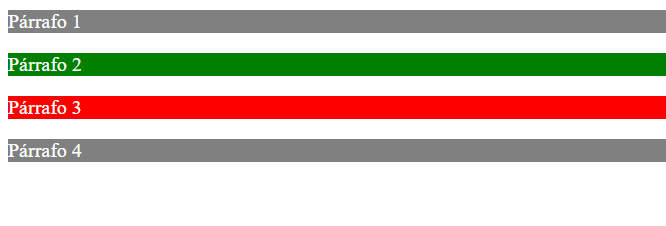
\includegraphics[width=12cm]{ss/tipos de estilos.png}
    \end{center}
\end{figure}

Vemos que hay cuatro párrafos, a cada uno tiene un estilo diferente: el párrafo 1 no tiene ni identificador ni clase, por lo que el estilo a aplicar es el de las etiquetas \textbf{p}; el párrafo 2 tiene el identificador "intro", por lo que el estilo a aplicar es el de dicho identificador; el párrafo 3 tiene la clase "cuerpo", por lo que el estilo a aplicar es el de dicha clase; el párrafo 4 está contenido dentro de una etiqueta \textbf{div}, la cual tiene el identificador y clase anteriormente mencionados, por lo que debemos considerar el orden de prioridad de los selectores CSS y HTML, por lo que el estilo a aplicar es el de las etiquetas \textbf{p}.


\subsection{Selectores descendentes}

Podemos aplicar un estilo a una etiqueta contenida dentro de otra que posee un estilo definido (un identificador, una clase o estilo de etiqueta), es decir, clase dentro de clase, identificador dentro de un identificador, clase dentro de identificador o viceversa, miremos un ejemplo (\textit{Figura \ref{fig: 2}}):
\begin{lstlisting}
estilos.css
    #intro .primero em {
        color: pink;
        background-color: gray;
    }

prueba.html
    <div id="intro">
        <p class="primero"><em>Párrafo 1</em> dentro del div</p>
    </div>
    <p class="primero">Párrafo 2 fuera del div.</p>
    <p>Párrafo 3 fuera del div</p>
\end{lstlisting}
\begin{figure}[H]
    \begin{center}
        \caption{Selectores descendentes}
        \label{fig: 2}
        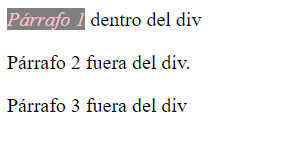
\includegraphics[width=6cm]{ss/selectores descendente.png}
    \end{center}
\end{figure}


\subsection{Comentarios}

Para comentar una o varias líneas de código en CSS se debe escribir los caracteres \textbf{/*} al comienzo o primer línea y \textbf{*/} al final o última línea de código.
\begin{lstlisting}
    /* Esto es un comentario. */

    /* Todo este estilo está comentado.
    p {
        color: red;
    } */
    
    #intro .primero em {
    color: pink;
    background-color: gray;
}
\end{lstlisting}



\section{Formas de aplicar estilos CSS}

Los estilos CSS pueden ser aplicados de tres maneras sencillas:


\subsection{Inline}

Implica aplicar el estilo mediante la atributo HTML \textbf{style}, dentro de sus dos comillas, asignamos las propiedades CSS de estilo que la etiqueta u objeto HTML tendrá, únicamente esta etiqueta, no el resto del mismo tipo.
\begin{lstlisting}
    <html>
        <head>
            <title>Prueba</title>
        </head>
        <body>
            <!-- Estilo Inline. -->
            <p style="color: white; background-color: gray;">Hola </p>
            <p>mundo.</p>
        </body>
    </html>
\end{lstlisting}

En el ejemplo anterior, solamente la primer etiqueta tendría un estilo definido.


\subsection{Embedded o Internal}

Contrario a la forma \textit{Inline}, donde se le aplica un estilo a una sola etiqueta, la forma \textbf{Embedded} crea un estilo dentro de la estructura HTML y se le puede aplicar a cuantas etiquetas se desee. Estos estilos internos son creados en la cabecera de la estructura del documento, utilizando la etiqueta \textbf{style}.
\begin{lstlisting}
    <html>
        <head>
            <title>Prueba</title>
            <!-- Estilo Embedded. -->
            <style>
                p {
                    color: white;
                    background-color> gray;
                }
            </style>
        </head>
        <body>
            <p>Hola </p>
            <p>mundo.</p>
        </body>
    </html>
\end{lstlisting}

En el ejemplo anterior, ambas etiquetas \textbf{p} tienen un mismo estilo definido. Es recomendable utilizar estilos internos cuando una sola página de un sitio web tiene un estilo único.


\subsection{External}

Con este método, debemos contar con un archivo con extensión \textbf{.css} en nuestro directorio y lo enlazamos a nuestro documento HTML mediante la siguiente etiqueta:
\begin{center}
    \textit{<link href="ejemplo.css" rel="stylesheet">}
\end{center}

Veamos un ejemplo:
\begin{lstlisting}
/* Estilo External. */
ejemplo.css
    p {
        color: white;
        background-color: gray;
    }

prueba.html
    <html>
        <head>
            <title>Prueba</title>
            <!-- Enlaza hoja de estilos al documentl HTML. -->
            <link href="ejemplo.css" rel="stylesheet">
        </head>
        <body>
            <p>Hola </p>
            <p>mundo </p>
            <p>estoy probando estilos CSS.</p>
        </body>
    </html>
\end{lstlisting}

Así, todos los cambios que hagamos a la hoja de estilos en su propio archivo se verá reflejado en el sitio web, siempre y cuando esta hoja de estilos esté ligada a la página.



\section{Herencia}

Al igual que otros lenguajes con un enfoque distinto, CSS aplica herencia a los elementos o etiquetas contenidas dentro de una que ya tenga un estilo definido, veamos como funciona esto:
\begin{lstlisting}
estilos.css
    body {
        color: red;
    }

prueba.html
    <p>Hola </p>
    <p>mundo </p>
    <p>estoy probando estilos CSS.</p>
\end{lstlisting}

En el ejemplo, ninguna etiqueta \textbf{p} tiene estilo definido, por lo que se les aplica el estilo de su etiqueta padre \textbf{body}.
\begin{lstlisting}
estilos.css
    body {
        color: red;
    }
    p {
        color: blue;
    }

prueba.html
    <p>Hola </p>
    <p>mundo </p>
    <p>estoy probando estilos CSS.</p>
\end{lstlisting}

Se creamos un estilo para las etiquetas \textbf{p} con un color de texto distinto, a estas etiquetas se les aplicará el estilo diseñado para ellas, en vez del estilo de su padre \textbf{body}, por lo que podemos concluir que \textbf{los estilos de los hijos de etiquetas tienen prioridad sobre sus padres}.

\section{Trabajando con texto}


\subsection{Fuentes}

La propiedad \textbf{font-family} (familia de fuentes) de CSS permite establecer la fuente (tipo de letra) de un elemento o etiqueta. La \textit{Tabla \ref{tab: 1}} contiene los dos tipos de familias de fuentes:
\begin{table}[H]
    \centering
    \caption{Tipos de familias de fuentes}
    \label{tab: 1}
    \begin{tabular}{c c}
        \hline
        \textbf{Generic family} & \textbf{Font family} \\
        \hline
        \multirow{2}{5cm}{Serif}                & Times New Roman \\
        & Georgia \\
        \multirow{2}{5cm}{Sans - serif}  & Arial \\
        & Verdana \\
        \multirow{2}{5cm}{Monospace}     & Courier New \\
        & Lucida Console \\
        \hline
    \end{tabular}
\end{table}

Las \textbf{familias genéricas} (o generic family) son un grupo de familias de fuentes, es decir, un grupo de fuentes, mientras que la familia de fuentes (o family font) es una fuente o tipo de letra que se puede utilizar.

Asignemos algunas fuentes a algunos párrafos y veamos el resultado en la \textit{Figura \ref{fig: 3}}:
\begin{lstlisting}
estilos.css
    /* Define distintas clases que almacenan las distintas fuentes. */
    .serif {
        /* Si fuente "Times New Roman" no está disponible, prueba con Times, si
         esta tampoco, con alguna parecida de la familia serif. */
        font-family: "Times New Roman", Times, serif;
    }
    .sansserif {
        font-family: Helvetica, Arial, sans-serif;
    }
    .monospace {
        font-family: "Courier New", Courier, monospace;
    }
    .cursive {
        font-family: Florence, cursive;
    }
    .fantasy {
        font-family: Blippo, fantasy;
    }
    .systemui {
        font-family: system-ui, -apple-system, BlinkMacSystemFont, 'Segoe UI', Roboto, Oxygen, Ubuntu, Cantarell, 'Open Sans', 'Helvetica Neue', sans-serif;
    }

prueba.html
    <p class="serif">Escrito con Serif.</p>
    <p class="sansserif">Escrito con Sans-Serif.</p> 
    <p class="monospace">Escrito con Monospace.</p> 
    <p class="cursive">Escrito con Cursive.</p> 
    <p class="fantasy">Escrito con Fantasy.</p>
    <p class="systemui">Escrito con System UI.</p>
\end{lstlisting}
\begin{figure}[H]
    \centering
    \caption{Uso de fuentes}
    \label{fig: 3}
    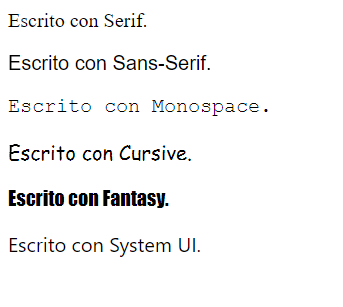
\includegraphics[width=6cm]{ss/fuentes.png}
\end{figure}

Como podemos ver, en el ejemplo anterior, si la fuente que deseamos no está disponible, podemos cargar otra deseada, si tampoco está disponible, podemos probar con alguna similar dentro de una familia, separado por comas (,); el ejemplo solamente prueba con dos fuentes antes de acudir a una familia, pero pueden ser más (no olvide que los nombres que son escritos con más de una palabra deben ser encerrados entre dobles comillas).

Una buena práctica es asignarle a todo el sitio web (body) una fuente genérica de respaldo, es decir, si queremos que todo nuestro sitio tenga la fuente de Google, pero por algún motivo, esta no está disponible (por la misma empresa o por una falla con el internet o máquina del cliente), podamos cargar otra fuente deseada y evitar un error de lectura. Lo anterior se resuelve como lo vimos en el ejemplo, poniendo diversas fuentes separadas por comas, para al final, poner una familia genérica.


\subsection{Tamaño de fuente}

La propiedad \textbf{font-size} de CSS permite establecer el tamaño de fuente del texto de un elemento o etiqueta. Una de las formas de hacer grande o pequeña el tamaño de fuente es por medio de \textbf{palabras clave}, tales como:
\begin{itemize}
    \item \textbf{small} (\textbf{smaller}, \textbf{x-small}, \textbf{xx-small}).
    \item \textbf{medium}.
    \item \textbf{large} (\textbf{larger}, \textbf{x-larger}, \textbf{xx-larger}).
    \item \textbf{inherit}, \textbf{initial} y \textbf{unset}.
\end{itemize}

Este método evita que el usuario varie el tamaño de la fuente, de esta forma, evitando que afecte la apariencia del sitio web. Un ejemplo y su resultado (\textit{Figura \ref{fig: 4}}):
\begin{lstlisting}
estilos.css
    /* Define distintas clases con tamaño de fuente distintas. */
    .small {
        font-size: small;
    }
    .medium {
        font-size: medium;
    }
    .large {
        font-size: large;
    }
    .xlarge {
        font-size: x-large;
    }

prueba.html
    <p class="small">Escrito pequeño.</p>
    <p class="medium">Escrito mediano.</p> 
    <p class="large">Escrito grande.</p> 
    <p class="x-large">Escrito muy grande.</p>
\end{lstlisting}
\begin{figure}[H]
    \centering
    \caption{Cambiando el tamaño de fuente}
    \label{fig: 4}
    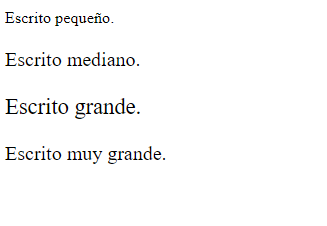
\includegraphics[width=6cm]{ss/fuentes-tam.png}
\end{figure}

La otra forma de definir el tamaño de fuente es mediante \textbf{Longitudes}: \textbf{px}, \textbf{em} o \textbf{porcentaje} (\%), la primera permite precisión en cuanto a píxeles en pantalla, mientras que la segunda permite cambio de tamaño en buscadores, pruebe ambas longitudes con zoom en su buscador para ver cómo funcionan y si se mantienen legibles (recuerde que 1em es igual a píxeles/16).
\begin{center}
    \textit{
        // Ambos tamaños son el mismo. \\
        font-size: 20px; \\
        font-size: 1.25em; \\
    }
\end{center}


\subsection{Estilo de fuente}

La propiedad \textbf{font-style} (estilo de fuente) permite aplicar un estilo de letra a la fuente, los valores que acepta esta propiedad son:
\begin{itemize}
    \item \textbf{normal}: texto sin ningún tipo de estilo (ni negrita).
    \item \textbf{italic}: texto en cursiva (lo mismo que la etiqueta \textbf{i}).
    \item \textbf{oblique}: texto como \textit{italic}, pero un poco más redonda (no es soportada por algunos buscadores).
    \item \textbf{oblique \textit{$<$ángulo$>$}}: texto como \textit{italic}, pero se le puede añadir un ángulo de inclinación al texto, esta propiedad no es muy soportada por los buscadores, los valores que puede recibir van de -90 a 90 deg.
    \item \textbf{inherit}, \textbf{initial} y \textbf{unset}.
\end{itemize}

Veamos un ejemplo y su resultado (\textit{Figura \ref{fig: 5}}):
\begin{lstlisting}
estilos.css
    /* Define distintas clases con estilos de fuente distintas. */
    .normal {
        font-style: normal;
    }
    .italic {
        font-style: italic;
    }
    .oblique {
        font-style: oblique;
    }

prueba.html
    <p class="normal">Escrito normal.</p>
    <p class="italic">Escrito italic.</p>
    <p class="oblique">Escrito oblique.</p>
\end{lstlisting}
\begin{figure}[H]
    \centering
    \caption{Cambiando el estilo de fuente}
    \label{fig: 5}
    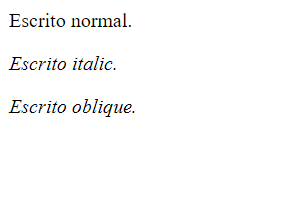
\includegraphics[width=6cm]{ss/fuentes-style.png}
\end{figure}

¿Porqué requeriría de esto si ya lo puedo conseguir con las etiquetas de HTML?, bueno, podemos aplicar un estilo de fuente distinto dinámicamente, por ejemplo, al dar un clic en un botón, un texto pasa de negrita a normal, normal a cursiva, etc.


\subsection{Grosor de fuente}

La propiedad\textbf{font-weight} (peso de fuente literalmente) de CSS permite establecer el grosor de fuente del texto de un elemento o etiqueta. Acepta los siguientes valores:
\begin{itemize}
    \item \textbf{normal}: texto normal con grosor predeterminado.
    \item \textbf{bold}: texto con un grosor mayor a \textit{normal} (como la etiqueta \textbf{b} o \textbf{stronger}).
    \item \textbf{bolder}: texto con un grosor mayor a \textit{bold}.
    \item \textbf{lighter}: texto con grosor menor a \textit{normal}.
    \item \textbf{inherit}, \textbf{initial} y \textbf{unset}.
\end{itemize}

Veamos un ejemplo y su resultado (\textit{Figura \ref{fig: 6}}):
\begin{lstlisting}
estilos.css
    /* Define distintas clases con grosores de fuente distintas. */
    .lighter {   
        font-weight: lighter;
    }
    .bold {   
        font-weight: bold;
    }
    .bolder {
        font-weight: bolder;
    }

prueba.html
    <p class="lighter">Escrito lighter.</p>
    <p class="bold">Escrito bold.</p>
    <p class="bolder">Escrito bolder.</p>
\end{lstlisting}
\begin{figure}[H]
    \centering
    \caption{Cambiando el grosor de fuente}
    \label{fig: 6}
    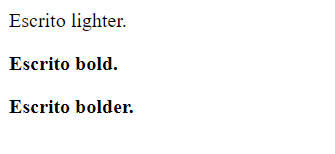
\includegraphics[width=6cm]{ss/fuentes-weight.png}
\end{figure}

Esta propiedad puede ser definida con valores enteros del 100 (ligero) a 900 (grueso), de acuerdo a como lo necesitemos. El valor 400 tiene el mismo grosor que el valor \textit{normal}, mientras que 700 tiene el mismo grosor que el valor \textit{bold}.
\begin{lstlisting}
    estilos.css
    /* Define distintas clases con grosores de fuente en valores. */
    .ligerito {   
        font-weight: 300;
    }
    .gruesesote {   
        font-weight: 850;
    }
\end{lstlisting}


\subsection{Variación de fuente}

La propiedad \textbf{font-variant} (variación de fuente) de CSS permite encoger ligeramente un texto de un elemento o etiqueta. Acepta los siguientes valores:
\begin{itemize}
    \item \textbf{normal}: texto con tamaño y estilo predeterminado.
    \item \textbf{small-caps}: texto encogido ligeramente y lo pasa a mayúsculas, tiene otros parámetros consecuentes que afectan al resultado final.
    \item \textbf{common-ligatures}: texto con tamaño predeterminado, pero con un espacio mayor entre letra y letra, tiene otros parámetros consecuentes que afectan al resultado final.
    \item \textbf{inherit}, \textbf{initial} y \textbf{unset}.
\end{itemize}

Veamos un ejemplo y su resultado (\textit{Figura \ref{fig: 7}}):
\begin{lstlisting}
estilos.css
    /* Define distintas clases con variaciones de fuente distintas. */
    .normal {
        font-variant: normal;
    }
    .small {
        font-variant: small-caps;
    }

prueba.html
    <p class="normal">Escrito normal.</p>
    <p class="small">Escrito small-caps.</p>
\end{lstlisting}
\begin{figure}[H]
    \centering
    \caption{Cambiando la variación de fuente}
    \label{fig: 7}
    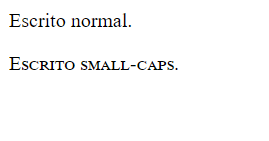
\includegraphics[width=6cm]{ss/fuentes-var.png}
\end{figure}


\subsection{Alineando texto horizontalmente}

La propiedad \textbf{text-align} de CSS permite establecer la alineación horizontal del texto de un objeto o etiqueta. Por defecto, el texto está alineado a la izquierda, pero también acepta los siguientes valores:
\begin{itemize}
    \item \textbf{start} o \textbf{left}: por defecto, alinea a la izquierda.
    \item \textbf{end} o \textbf{right}: alinea a la derecha.
    \item \textbf{center}: alinea al centro.
    \item \textbf{justify}: alinea a la izquierda y derecha.
    \item \textbf{inherit}, \textbf{initial} y \textit{unset}.
\end{itemize}

Veamos el siguiente ejemplo y su resultado (\textit{Figura \ref{fig: 8}}):
\begin{lstlisting}
estilos.css
    /* Define distintas clases con alineaciones de texto distintas. */
    .izq {
        text-align: left;
    }
    .der {
        text-align: right;
    }
    .cen {
        text-align: center;
    }
    .jus {
        text-align: justify;
    }

prueba.html
    <p class="izq">Lorem ipsum dolor sit amet, consectetur adipiscing elit, sed do eiusmod tempor incididunt ut
                labore et dolore magna aliqua. Ut enim ad minim veniam, quis nostrud exercitation ullamco laboris nisi ut
                aliquip ex ea commodo consequat</p>
    <p class="der">Lorem ipsum dolor sit amet, consectetur adipiscing elit, sed do eiusmod tempor incididunt ut
                labore et dolore magna aliqua. Ut enim ad minim veniam, quis nostrud exercitation ullamco laboris nisi ut
                aliquip ex ea commodo consequat</p>
    <p class="cen">Lorem ipsum dolor sit amet, consectetur adipiscing elit, sed do eiusmod tempor incididunt ut
                labore et dolore magna aliqua. Ut enim ad minim veniam, quis nostrud exercitation ullamco laboris nisi ut
                aliquip ex ea commodo consequat</p>
    <p class="jus">Lorem ipsum dolor sit amet, consectetur adipiscing elit, sed do eiusmod tempor incididunt ut
                labore et dolore magna aliqua. Ut enim ad minim veniam, quis nostrud exercitation ullamco laboris nisi ut
                aliquip ex ea commodo consequat</p>
\end{lstlisting}
\begin{figure}[H]
    \centering
    \caption{Cambiando la alineación de texto}
    \label{fig: 8}
    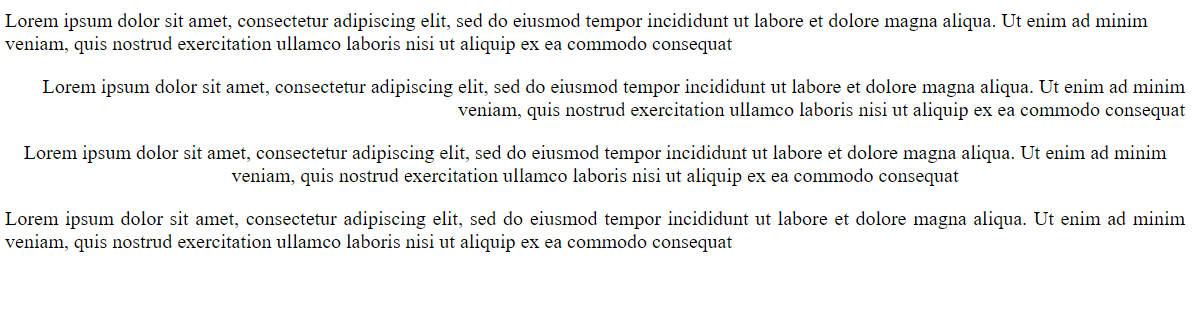
\includegraphics[width=14cm]{ss/fuentes-align.png}
\end{figure}


\subsection{Alineando texto verticalmente}

La propiedad \textbf{vertical-align} de CSS permite establecer la alineación vertical del texto de un objeto o etiqueta. Por defecto, el texto está alineado en la parte superior de la página, pero también acepta los valores:
\begin{itemize}
    \item \textbf{top}: alinea el tope del elemento con el tope de la línea entera o su contenedor.
    \item \textbf{bottom}: alinea la base del elemento con la base de la línea entera o su contenedor.
    \item Valores con respecto el elemento padre:
    \begin{itemize}
        \item \textbf{baseline}: alinea la base del elemento con la base de su elemento padre.
        \item \textbf{sub}: alinea la base del elemento con la base del subíndice de su elemento padre.
        \item \textbf{super}: alinea la base del elemento con la base del superíndice de su elemento padre.
        \item \textbf{text-top}: alinea el tope del elemento con el tope de la letra de su elemento padre.
        \item \textbf{text-bottom}: alinea la base del elemento con la base de la letra de su elemento padre.
        \item \textbf{middle}: alinea la mitad del elemento con la base más una porción X del alto de su elemento padre.
    \end{itemize}
    \item \textbf{inherit}, \textbf{initial} y \textit{unset}.
\end{itemize}

Veamos el siguiente ejemplo con una tabla y su resultado (\textit{Figura \ref{fig: 9}}):
\begin{lstlisting}
estilos.css
    /* Define distintas clases con alineaciones verticales de texto distintas. */
    .cima {
        vertical-align: top;
    }
    .medio {
        vertical-align: middle;
    }
    .fondo {
        vertical-align: bottom;
    }

prueba.html
    <table border="1" cellpadding="2" cellspacing="0" style="height: 150px;">
        <tr>
            <td class="cima">Top</td>
            <td class="medio">Middle</td>
            <td class="fondo">Bottom</td>
        </tr>
    </table>
\end{lstlisting}
\begin{figure}[H]
    \centering
    \caption{Cambiando la alineación vertical de texto 1}
    \label{fig: 9}
    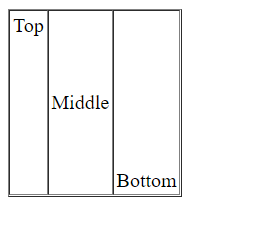
\includegraphics[width=5cm]{ss/fuentes-align-v1.png}
\end{figure}

Lamentablemente, los palabras clave anteriormente mencionadas solamente aplican para las etiquetas \textbf{table}, sin embargo, podemos utilizar otras palabras reservadas como valores para otras etiquetas con esta propiedad, los cuales son: \textbf{baseline}, \textbf{sub}, \textbf{super} y \textbf{Longitudes} (\%, px, pt, cm, em, etc.). Veamos un ejemplo continuación (\textit{Figura \ref{fig: 10}}).
\begin{lstlisting}
estilos.css
    /* Define distintas clases con alineaciones verticales de texto distintas. */
    .baseline {
        vertical-align: baseline;
    }
    .sub {
        vertical-align: sub;
    }
    .super {
        vertical-align: super;
    }
    .pixel {
        vertical-align: 10px;
    }

prueba.html
    <p>Este texto tiene una palabra <span class="baseline">baseline</span>.</p>
    <p>Este texto tiene una palabra <span class="sub">sub</span>.</p>
    <p>Este texto tiene una palabra <span class="super">super</span>.</p>
    <p>Este texto tiene una palabra <span class="pixel">subida 10 píxeles</span>.</p>
\end{lstlisting}
\begin{figure}[H]
    \centering
    \caption{Cambiando la alineación vertical de texto 2}
    \label{fig: 10}
    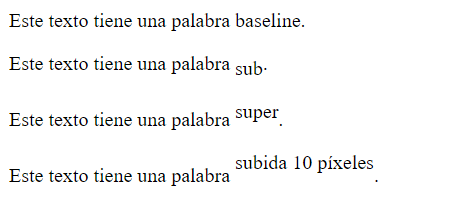
\includegraphics[width=9cm]{ss/fuentes-align-v2.png}
\end{figure}

\textit{Nota}: el ejemplo anterior aplicó a un párrafo (\textbf{p} y \textbf{span}), pero requiere de más instrucciones (propiedades) para otras etiquetas.


\subsection{Color de texto}

La propiedad \textbf{color} de CSS permite establecer un color determinado al texto de un objeto o etiqueta. Una de las formas de aplicar color al texto es utilizando las palabras claves con los nombres de los colores, por ejemplo: \textit{red}, \textit{green}, \textit{blue}, etc. Veamos un ejemplo rápido (\textit{Figura \ref{fig: 11}}):
\begin{lstlisting}
estilos.css
    /* Define una clase que asigna el color rojo al texto. */
    .colores {
        color: red;
    }

prueba.html
    <p class="colores">Escrito con color rojito.</p>
    <p>Escrito con el color predefinido (negro).</p>
\end{lstlisting}
\begin{figure}[H]
    \centering
    \caption{Cambiando el color del texto}
    \label{fig: 11}
    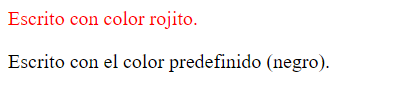
\includegraphics[width=9cm]{ss/fuentes-color.png}
\end{figure}

La otra forma de asignar colores es por medio de valores hexadecimales, compuesto por un \# al inicio y seis caracteres, que van de o a F, o RGB, que define un valor de 0 a 255 para el rojo, verde y azul (Red, Green y Blue).
\begin{center}
    \textit{
        // Color blanco. \\
        color: \#FFFFFF; \\
        color: rgb(255, 255, 255); \\
    }
\end{center}


\subsection{Decoración del texto}

La propiedad \textbf{text-decoration} de CSS permite establecer una decoración al texto de un objeto o etiqueta. Algunos de los valores aceptados son:
\begin{itemize}
    \item \textbf{none}: establece un texto regular o normal, sin estilo ni decoración.
    \item \textbf{overline}: establece una línea horizontal encima del texto.
    \item \textbf{underline}: establece una línea horizontal debajo del texto.
    \item \textbf{line-through}: establece una línea horizontal en medio del texto, es decir, lo tacha (sustituye la etiqueta \textbf{s} de HTML).
    \item \textbf{inherit}, \textbf{initial} y \textit{unset}.
\end{itemize}

Veamos un ejemplo rápido (\textit{Figura \ref{fig: 12}}):
\begin{lstlisting}
estilos.css
    /* Define una clase que asigna una decoración al texto distinta. */
    .none {
        text-decoration: none;
    }
    .inherit {
        text-decoration: inherit;
    }
    .overline {
        text-decoration: overline;
    }
    .underline {
        text-decoration: underline;
    }
    .line-through {
        text-decoration: line-through;
    }
    
prueba.html
    <p class="none">Escrito predeterminado.</p>
    <p class="inherit">Escrito que hereda el estilo de su padre.</p>
    <p class="overline">Escrito que tiene una línea encima.</p>
    <p class="underline">Escrito que tiene una línea debajo.</p>
    <p class="line-through">Escrito que está tachado.</p>
\end{lstlisting}
\begin{figure}[H]
    \centering
    \caption{Cambiando la decoración del texto}
    \label{fig: 12}
    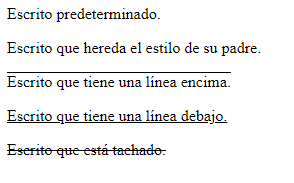
\includegraphics[width=9cm]{ss/fuentes-deco.png}
\end{figure}

Esta propiedad tiene otras propiedades consecuentes, como lo son un color, estilo o grosor, por ejemplo:
\begin{center}
    \textit{text-decoration: underline dotted red;}
\end{center}

Los \textbf{colores} ya sabemos que pueden ser utilizamos mediante palabras reservadas o códigos hexadecimales, los valores para la propiedad \textbf{estilo} son similares o iguales a los valores utilizados para estilizar los bordes de tablas (\textit{dotted}, \textit{solid}, \textit{double}, etc), los valores para la propiedad \textbf{grosor} son \textbf{auto} y \textbf{from-font}.


\subsection{Indentación del texto}

La propiedad \textbf{text-indent} de CSS permite establecer una indentación al texto de un objeto o etiqueta. Acepta \textbf{Longitudes} como valor para definir el espacio del lado izquierdo antes de comenzar el texto (px, pt, cm, em, \%, \textbf{inherit}, \textbf{initial} y \textbf{unset}, valores negativos, etc.). Veamos un ejemplo rápido (\textit{Figura \ref{fig: 13}}):
\begin{lstlisting}
estilos.css
    /* Define una clase que asigna una indentación al texto. */
    p {
        text-indent: 20px;
    }
    
prueba.html
    <p>Lorem ipsum dolor sit amet, consectetur adipiscing elit, sed do eiusmod tempor 
            incididunt ut labore et dolore magna aliqua. Ut enim ad minim veniam, quis 
            nostrud exercitation ullamco laboris nisi ut aliquip ex ea commodo consequat</p>
\end{lstlisting}
\begin{figure}[H]
    \centering
    \caption{Cambiando la indentación del texto}
    \label{fig: 13}
    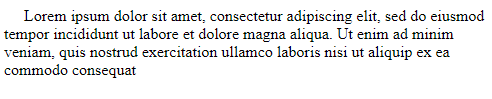
\includegraphics[width=12cm]{ss/fuentes-indent.png}
\end{figure}


\subsection{Sombra del texto}

La propiedad \textbf{text-shadow} de CSS permite establecer una sombra proveniente del centro del texto de un objeto o etiqueta. Posee cuatro parámetros: distancia del centro del texto con respecto al eje X (horizontal), distancia del centro del texto con respecto al eje Y (vertical), lo borroso o difuminado de la sombra y su color; todos estos parámetros \textbf{no} van separados por comas. Veamos un ejemplo rápido (\textit{Figura \ref{fig: 14}}):
\begin{lstlisting}
estilos.css
    /* Define una clase que asigna una una sombra con color al texto. */
    .sombrita {
        color: blueviolet;
        /* La sombra se proyecta en diagonal 5 y 5 píxeles hacía la abajo y derecha,
           está difuminada 5 píxeles y es de color azul. */
        text-shadow: 5px 5px 5px blue;
    }
    
prueba.html
    <h1 class="sombrita">Este texto tiene sombra</h1>
\end{lstlisting}
\begin{figure}[H]
    \centering
    \caption{Agregando sombra al texto}
    \label{fig: 14}
    
\includegraphics[width=7cm]{ss/fuentes-shadow.png}
\end{figure}

Como podemos suponer, los valores de los atributos pueden ser negativos y las distintas \textbf{Longitudes} permitidas por CSS, podemos utilizar valores hexadecimales o RGB para establecer el color de la sombra y podemos establecer múltiples sombras a un texto, simplemente separamos este grupo de parámetros por una coma y ponemos otro grupo de cuatro:
\begin{center}
    \textit{text-shadow: 5px 5px 5px blue, rgba(0,0,255,1) -1px -2px 0.5em;}
\end{center}

Un valor que también se puede poner es \textbf{transparent}, que hace transparente una sombra, además de \textbf{inherit}, \textbf{initial} y \textit{unset}.


\subsection{Transformación del texto}

La propiedad \textbf{text-transform} de CSS permite configurar la forma en la que aparecen las mayúsculas y minúsculas en el texto de un objeto o etiqueta. Algunos valores que acepta esta propiedad son:
\begin{itemize}
    \item \textbf{none}: aplica un estilo normal o predeterminado a un texto.
    \item \textbf{capitalize}: pone mayúsculas a cada palabra de un texto.
    \item \textbf{uppercase}: vuelve todo el texto mayúscula.
    \item \textbf{lowercase}: vuelve todo el texto minúscula.
    \item \textbf{inherit}, \textbf{initial} y \textit{unset}.
\end{itemize}

Veamos un ejemplo rápido (\textit{Figura \ref{fig: 15}}):
\begin{lstlisting}
estilos.css
    /* Define una clase que cambia el orden de minúsculas y mayúsculas del texto. */
    .none {
        text-transform: none;
    }
    .capitalize {
        text-transform: capitalize;
    }
    .uppercase {
        text-transform: uppercase;
    }
    .lowercase {
        text-transform: lowercase;
    }
    
prueba.html
    <p class="none">eScRiTO nONe</p>
    <p class="capitalize">eScRiTO CaPiTaLiZe</p>
    <p class="uppercase">eScRiTO upperCASE</p>
    <p class="lowercase">eScRiTO LOWERcase</p>
\end{lstlisting}
\begin{figure}[H]
    \centering
    \caption{Cambiando las mayúsculas y minúsculas del texto}
    \label{fig: 15}
    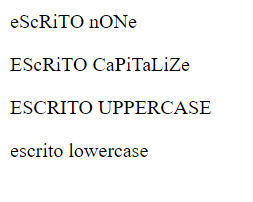
\includegraphics[width=5cm]{ss/fuentes-upper.png}
\end{figure}


\subsection{Espaciado entre letras}

La propiedad \textbf{letter-spacing} de CSS permite configurar el espaciado entre carácter y carácter de un texto de un objeto o etiqueta. Algunos valores que acepta esta propiedad son:
\begin{itemize}
    \item \textbf{normal}: no agrega ningún espaciado entre caracteres.
    \item \textbf{inherit}, \textbf{initial} y \textit{unset}.
\end{itemize}

Veamos un ejemplo rápido (\textit{Figura \ref{fig: 16}}):
\begin{lstlisting}
estilos.css
    /* Define una clase que cambia el espaciado de caracteres del texto. */
    .normal {
        letter-spacing: normal;
    }
    .esp {
        letter-spacing: 5px;
    }
        
prueba.html
    <p class="normal">Espaciado normal.</p>
    <p class="esp">Espaciado de 5px.</p>
\end{lstlisting}
\begin{figure}[H]
    \centering
    \caption{Cambiando el espaciado de caracteres del texto}
    \label{fig: 16}
    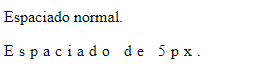
\includegraphics[width=7cm]{ss/fuentes-spacing.png}
\end{figure}

\textit{Nota}: letter-spacing acepta valores negativos.


\subsection{Espaciado entre palabras}

La propiedad \textbf{word-spacing} de CSS permite configurar el espaciado entre palabras de un texto de un objeto o etiqueta. Así como con la propiedad anterior, esta acepta los valores \textbf{normal}, una \textbf{Longitud} (\%, px, pt, cm, em, etc.), \textbf{inherit}, \textbf{initial} y \textit{unset}. Veamos un ejemplo rápido (\textit{Figura \ref{fig: 17}}):
\begin{lstlisting}
estilos.css
    /* Define una clase que cambia el espaciado de palabras del texto. */
    .normal {
        word-spacing: normal;
    }
    .esp {
        word-spacing: 20px;
    }
        
prueba.html
    <p class="normal">Este párrafo tiene un espaciado de palabras normal.</p>
    <p class="esp">Este párrafo tiene un espaciado de palabras de 20 píxeles.</p>
\end{lstlisting}
\begin{figure}[H]
    \centering
    \caption{Cambiando el espaciado de palabras del texto}
    \label{fig: 17}
    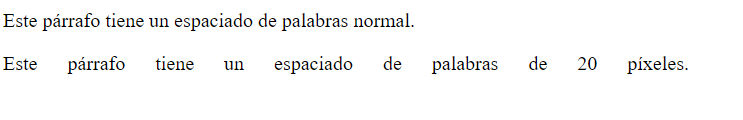
\includegraphics[width=14cm]{ss/fuentes-ws.png}
\end{figure}

\textit{Nota}: word-spacing acepta valores negativos.


\subsection{Manejo de espacios y saltos de línea}

La propiedad \textbf{white-space} de CSS permite configurar cómo son manejados los espacios en blanco y saltos de línea en textos, tanto en el código, como en el navegador cuando este cambia de tamaño, en otras palabras, maneja como se ajusta el texto cuando un elemento o etiqueta HTML sufre un cambio de tamaño Los valores que puede aceptar son los siguientes:
\begin{itemize}
    \item \textbf{normal}: el texto en código con secuencias de espacios y saltos de línea son reducidos a un solo espacio, manteniendo el texto dentro del espacio de la etiqueta que lo contiene.
    \item \textbf{nowrap}: trata los espacios y saltos de líneas como el valor \textit{normal}, pero el texto se sale del espacio de la etiqueta que lo contiene si esta no es lo suficientemente grande como para almacenarlo.
    \item \textbf{pre}: los múltiples espacios continuos se mantienen y los saltos de línea se dan con etiquetas \textbf{br} y con los caracteres de saltos de línea.
    \item \textbf{pre-wrap}: trata los espacios y saltos de líneas como el valor anterior, pero rellena con saltos de línea según sea necesario, para rellenar el contenedor que lo almacena.
    \item \textbf{pre-line}: trata los saltos de líneas como el valor anterior, pero la secuencia de espacios son reducidos a un solo espacio.
    \item \textbf{break-spaces}: idéntico al valor \textit{pre-wrap}, pero mantiene todos los espacios (incluidos los espacios al final de líneas) y secuencias de espacios.
\end{itemize}

La \textit{Tabla \ref{tab: 2}} muestra las diferentes situaciones donde podemos utilizar esta propiedad:
\begin{table}[H]
    \centering
    \caption{Usos de la propiedad \textit{white-space}}
    \label{tab: 2}
    \begin{tabular}{m{1.7cm} m{2cm} m{2.3cm} m{2cm} m{2cm} m{3cm}}
        \hline
        \parbox{1.7cm}{\raggedright} & \parbox{2cm}{\raggedright\textbf{Saltos de líneas}} & \parbox{2.3cm}{\raggedright\textbf{Espacios y \\tabulación}} & \parbox{2cm}{\raggedright\textbf{Ajuste de texto}} & \parbox{2cm}{\raggedright\textbf{Espacios al final}} & \parbox{3cm}{\raggedright\textbf{Separadores}} \\
        \hline
        \parbox{1.7cm}{\raggedright normal}       & \parbox{2cm}{\raggedright Se reducen} & \parbox{2.3cm}{\raggedright Se reducen} & \parbox{2cm}{\raggedright Se ajusta} & \parbox{2cm}{\raggedright Son removidos} & \parbox{3cm}{\raggedright Se cuelga} \\
        \hline
        \parbox{1.7cm}{\raggedright nowrap}       & \parbox{2cm}{\raggedright Se reducen}    & \parbox{2.3cm}{\raggedright Se reducen}    & \parbox{2cm}{\raggedright No se ajusta}  & \parbox{2cm}{\raggedright Son removidos} & \parbox{3cm}{\raggedright Se cuelga}    \\
        \hline
        \parbox{1.7cm}{\raggedright pre}          & \parbox{2cm}{\raggedright Se mantienen}  & \parbox{2.3cm}{\raggedright Se mantienen}  & \parbox{2cm}{\raggedright No se ajusta}  & \parbox{2cm}{\raggedright Se mantienen}  & \parbox{3cm}{\raggedright No se ajusta} \\
        \hline
        \parbox{1.7cm}{\raggedright pre-wrap}     & \parbox{2cm}{\raggedright Se mantienen}  & \parbox{2.3cm}{\raggedright Se mantienen}  & \parbox{2cm}{\raggedright Se ajusta}     & \parbox{2cm}{\raggedright Se cuelga}     & \parbox{3cm}{\raggedright Se cuelga}    \\
        \hline
        \parbox{1.7cm}{\raggedright pre-line}     & \parbox{2cm}{\raggedright Se mantienen}  & \parbox{2.3cm}{\raggedright Se reducen}    & \parbox{2cm}{\raggedright Se ajusta}     & \parbox{2cm}{\raggedright Son removidos} & \parbox{3cm}{\raggedright Se cuelga}    \\
        \hline
        \parbox{1.7cm}{\raggedright break-spaces} & \parbox{2cm}{\raggedright Se mantienen}  & \parbox{2.3cm}{\raggedright Se mantienen}  & \parbox{2cm}{\raggedright Se ajusta}     & \parbox{2cm}{\raggedright Se cuelga}     & \parbox{3cm}{\raggedright Se ajusta}    \\
        \hline
    \end{tabular}
\end{table}

Veamos un ejemplo rápido (\textit{Figura \ref{fig: 18}}):
\begin{lstlisting}
estilos.css
    /* Define una clase que manipula distinto los espaciados y saltos de líneas del texto. */
    /* Estilo de apoyo para visualizar mejor el ejemplo. */
    p {
        border-color: black;
        border-style: solid;
    }
    .normal {
        white-space: normal;
    }
    .nowrap {
        white-space: normal;
    }
    .pre {
        white-space: pre;
    }
    .pre-wrap {
        white-space: pre-wrap;
    }
    .pre-line {
        white-space: pre-line;
    }
    .break-spaces {
        white-space: break-spaces;
    }
        
prueba.html
    <p class="normal">Este párrafo             tiene
            un espaciado blanco              de palabras
            normal.
    </p>
    <p class="nowrap">Este párrafo             tiene
                un espaciado blanco              de palabras
                <i>nowrap</i>.
    </p>
    <p class="pre">Este párrafo             tiene
                 un espaciado blanco              de palabras
                  <i>pre</i>.
    </p>
    <p class="pre-wrap">Este párrafo             tiene
                un espaciado blanco              de palabras
                <i>pre-wrap</i>.
    </p>
    <p class="pre-line">Este párrafo             tiene
                un espaciado blanco              de palabras
                <i>pre-line</i>.
    </p>
    <p class="break-spaces">Este párrafo             tiene
                un espaciado blanco              de palabras
                <i>break-spaces</i>.
    </p>
\end{lstlisting}
\begin{figure}[H]
    \centering
    \caption{Cambiando el manejo de espacios y saltos de líneas del texto}
    \label{fig: 18}
    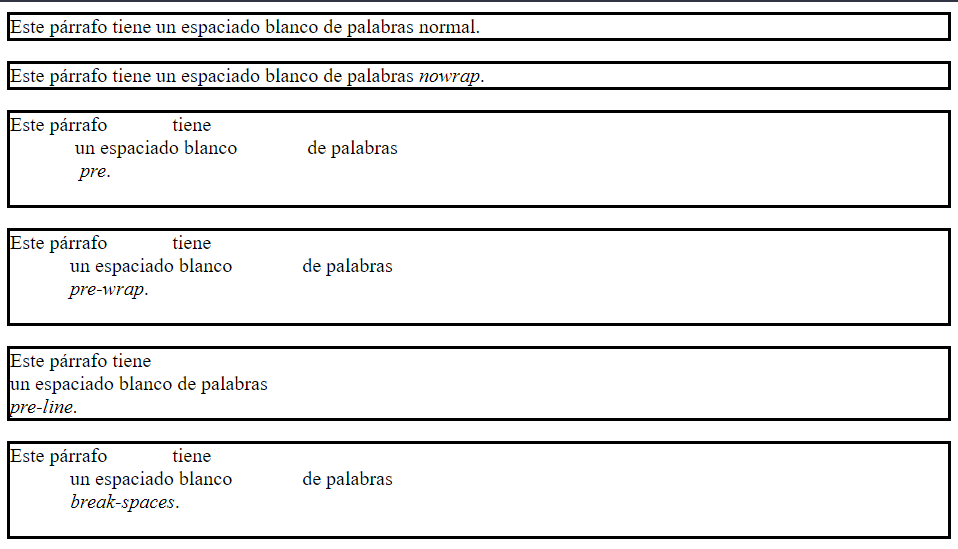
\includegraphics[width=14cm]{ss/fuentes-white-sp.png}
\end{figure}

\include{3.box model-estilizacion.tex}
\section{Posicionamiento}

Se refiere a la posibilidad de posicionar un elemento HTML en la página del sitio web. La propiedad para posicionar un elemento es \textbf{position}, la cual tiene algunos valores importantes a conocer:
\begin{itemize}
    \item \textbf{static}: se mantiene fijo según el flujo de elementos de la página, aún después de deslizarse hacía bajo en el sitio. Es es valor por defecto y no se puede posicionar fuera del flujo de elementos.
    \item \textbf{fixed}: se posiciona en una parte en específico de la página, aún después de deslizarse hacía abajo en el sitio, por lo que no sigue el flujo de elementos, esto puede provocar \textbf{superposición de elementos}.
    \item \textbf{relative}: se posiciona en una parte en específico de la página, pero se mantiene fija en dicha posición después de deslizar hacía abajo en el sitio (puede causar superposición de elementos).
    \item \textbf{absolute}: se posiciona en una parte en específico de la página, tomando como referencia la posición de su etiqueta padre más próxima, si no tiene, tomara esta referencia del documento en sí (body); se mantiene fija en dicha posición después de deslizar hacía abajo en el sitio (puede causar superposición de elementos).
\end{itemize}

Para posicionar un elemento en alguna parte en específico de la página, requerimos de las propiedad \textit{top}, \textit{left}, \textit{bottom}, \textit{right} y las \textit{unidades de valores}. Dejaremos un ejemplo sobre los posicionamientos de etiquetas y su resultado en la \textit{Figura \ref{fig: 25}}:
\begin{lstlisting}
estilos.css
    /* Se mantiene fijo en el flujo del documento. */
    .static p {
        position: static;
        /* Se ignoran las propiedades "top" y "left" debido a la posición estática. */
        top: 200px;
        left: 150px;
        width: 100px;
        height: 100px;
        background-color: red;
    }
    /* Se posiciona donde se desee, fuera del flujo del documento. */
    .fixed p {
        position: fixed;
        /* A 150px y 150px de la esquina superior izquierda. */
        top: 150px;
        left: 150px;
        width: 100px;
        height: 100px;
        background-color: blue;
        color: white;
    }
    /* Se posiciona donde se desee, dentro del flujo del documento. */
    .relative {
        position: relative;
        /* A 100px y 50px de la esquina superior izquierda. */
        top: 100px;
        left: 50px;
        width: 100px;
        height: 100px;
        background-color: coral;
    }
    /*
        Se posiciona donde se desee y con respecto a su etiqueta padre,
        en este caso, "body", fuera del flujo del documento.
    */
    .absolute {
        position: absolute;
        /* A 100px de la esquina superior izquierda. */
        top: 100px;
        width: 100px;
        height: 100px;
        background-color: darkgreen;
    }
    body {
        height: 5000px;
    }

prueba.html
    <div class="static">
        <p>Este párrafo tiene static position.</p>
    </div>
    <div class="fixed">
        <p>Este párrafo tiene fixed position.</p>
    </div>
    <div class="relative">
        <p>Este párrafo tiene relative position.</p>
    </div>
    <div class="absolute">
        <p>Este párrafo tiene absolute position.</p>
    </div>
\end{lstlisting}
\begin{figure}[H]
    \centering
    \caption{Diferencia entre valores de propiedad \textit{position}}
    \label{fig: 25}
    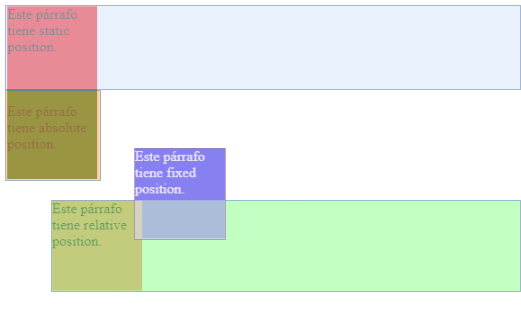
\includegraphics[width=14cm]{ss/position.png}
\end{figure}

Debe ejecutar este código en su buscador, ya que las diferencias visuales solamente se pueden apreciar cuando se desplaza sobre la página web.



\section{Floating}

La propiedad \textbf{float} de CSS permite que los elementos alrededor de otro "floten" o lo rodeen (usualmente utilizado en imágenes). Los valores que se aceptan son:
\begin{itemize}
    \item \textbf{left}: los elementos flotan a la izquierda.
    \item \textbf{right}: los elementos flotan a la derecha.
    \item \textbf{none}: los elementos no flotan (valor predeterminado).
    \item \textbf{inline-start}: los elementos flotan al principio de un contenedor o elemento padre.
    \item \textbf{inline-end}: los elementos flotan al final de un contenedor o elemento padre.
    \item \textbf{ihnerit}, \textbf{initial} y \textbf{unset}.
\end{itemize}

Los elementos que tiene la propiedad \textit{float} se posicionan en el extremo izquierdo o derecho (dependiendo si se estableció el valor \textit{left} o \textit{right} respectivamente) del contenedor donde están almacenados (body, div, section, etc.), y el resto de elementos los rodean. Dejaremos un ejemplo sobre los elementos flotantes y su resultado en la \textit{Figura \ref{fig: 26}}:
\begin{lstlisting}
estilos.css
    /* Muestra los elementos contenidos como bloques. */
    .block {
        display: block;
        height: 200px;
    }
    /* Los elementos flotan a la izquierda. */
    .left {
        float: left;
    }
    /* Los elementos flotan a la derecha. */
    .right {
        float: right;
    }

prueba.html
    <div class="block">
        <div class="left">
            <img src="https://www.zooplus.es/magazine/wp-content/uploads/2022/05/Cuanto-pesa-un-gato-2.jpeg"
            alt="https://images.unsplash.com/photo-1591871937631-2f64059d234f?ixlib=rb-4.0.3&ixid=MnwxMjA3fDB8MHxleHBsb3JlLWZlZWR8MXx8fGVufDB8fHx8&w=1000&q=80"
             width="200px" />
        </div>
        <p>Este párrafo flota al lado derecho de la imagen.</p>
    </div>
    <div class="block">
        <div class="right">
            <img src="https://www.zooplus.es/magazine/wp-content/uploads/2022/05/Cuanto-pesa-un-gato-2.jpeg"
            alt="https://images.unsplash.com/photo-1591871937631-2f64059d234f?ixlib=rb-4.0.3&ixid=MnwxMjA3fDB8MHxleHBsb3JlLWZlZWR8MXx8fGVufDB8fHx8&w=1000&q=80"
            width="200px" />
        </div>
        <p>Este párrafo flota al lado izquierdo de la imagen.</p>
    </div>
\end{lstlisting}
\begin{figure}[H]
    \centering
    \caption{Diferencia entre valores de propiedad \textit{float}}
    \label{fig: 26}
    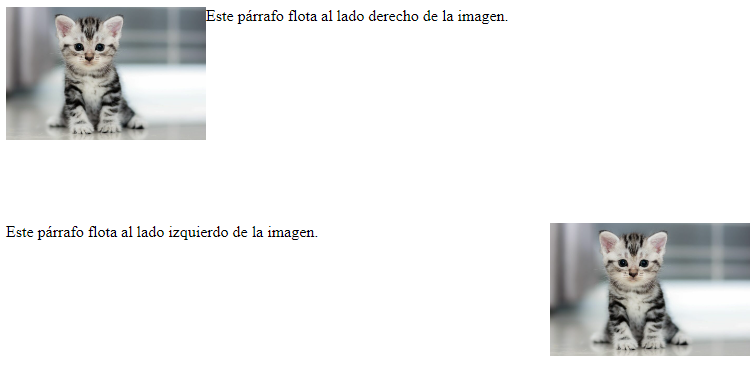
\includegraphics[width=14cm]{ss/float.png}
\end{figure}

En caso de que existan múltiples elementos con la propiedad \textit{float} uno al lado del otro, estos se posicionarán sin más uno enseguida del otro.



\section{Propiedades para la visualización de elementos}

Recordemos que todo elemento HTML es una caja, con su margen, \textit{padding}, borde y contenido; el buscador visualizará estos estos elementos de dos maneras principales:
\begin{itemize}
    \item \textbf{block-element}: elementos bloques, el buscador pondrá los elementos uno encima de otro (apilados), abarcando el 100\% del ancho de la página, a pesar de que el contenido de la etiqueta no lo abarque. Por lo general, muchas etiquetas tienen este tipo de visualización por defecto.
    \item \textbf{inline-elements}: elementos en línea, el buscador pondrá los elementos uno al lado del otro, ocupando solamente el ancho que requiera su contenido. Por lo general, las etiquetas \textbf{a} tienen este tipo de visualización por defecto.
\end{itemize}

Los dos conceptos anteriores servirán para explicar el ejemplo y figura del tema anterior, así como posteriores. La \textit{Figura \ref{fig: 27}} muestra la apariencia de ambas visualizaciones:
\begin{figure}[H]
    \centering
    \caption{Aspecto de las visualizaciones \textit{block} e \textit{inline}}
    \label{fig: 27}
    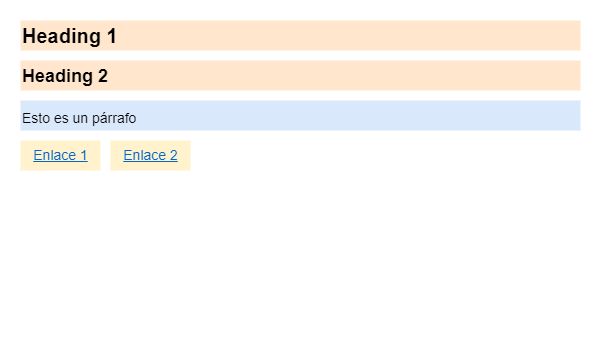
\includegraphics[width=12cm]{ss/display.png}
\end{figure}

Veremos entonces a continuación como modificar esta visualización con CSS.


\subsection{display}

La propiedad \textbf{display} de CSS acepta los siguientes valores:
\begin{itemize}
    \item \textbf{block}: visualiza los elementos HTML como elementos bloque, pudiendo cambiar su ancho y alto.
    \item \textbf{inline}: visualiza los elementos HTML como elementos en línea, no pudiendo cambiar su ancho y alto.
    \item \textbf{none}: no visualiza el elemento HTML, lo esconde, como si no estuviera presente, mostrando únicamente el contenedor que lo almacena.
    \item \textbf{inline-block}: visualiza los elementos HTML como elementos en línea, pero teniendo la posibilidad de asignar un ancho o alto al elemento.
\end{itemize}

Dejaremos un ejemplo sobre los posicionamientos de etiquetas y su resultado en la \textit{Figura \ref{fig: 28}}, inspeccionando cada elemento para que se note la diferencia entre todas:
\begin{lstlisting}
estilos.css
    /* Visualiza el elemento como bloque. */
    .block {
        display: block;
    }
    .block p {
        /* Hereda la visualización del bloque de su padre. */
        display: inherit;
        /* Establece tamaño al elemento. */
        width: 100px;
        height: 100px;
        background-color: red;
    }
    /* Visualiza el elemento como en línea. */
    .inline {
        display: inline;
    }
    .inline p {
        display: inherit;
        width: 100px;
        height: 100px;
        background-color: blue;
        color: white;
    }
    /* Visualiza el elemento como descartado. */
    .none {
        display: none;
    }
    /* Visualiza el elemento como bloque en línea. */
    .inline-block {
        display: inline-block;
    }
    .inline-block p {
        display: inherit;
        width: 100px;
        height: 100px;
        background-color: aqua;
    }

prueba.html
    <div class="block">
        <p>Este párrafo tiene block display.</p>
        <p>Este párrafo tiene block display.</p>
    </div>
    <div class="inline">
        <p>Este párrafo tiene inline display.</p>
        <p>Este párrafo tiene inline display.</p>
    </div>
    <div class="none">
        <p>Este párrafo no se incluirá en la visualización.</p>
    </div>
    <div class="inline-block">
        <p>Este párrafo tiene inline-block display.</p>
    </div>
\end{lstlisting}
\begin{figure}[H]
    \centering
    \caption{Diferencia entre valores de propiedad \textit{display}}
    \label{fig: 28}
    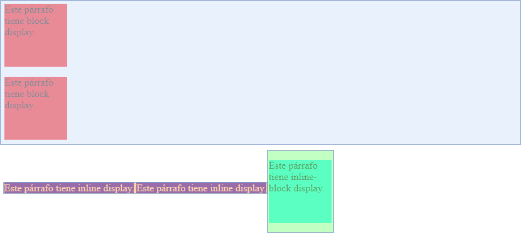
\includegraphics[width=14cm]{ss/prop-display.png}
\end{figure}

Vea que, a pesar de haber definido un tamaño para los elementos \textit{inline}(width=100px y height=100px), estos no sufren dichos cambios a su tipo de display, si tuvieran el valor \textit{block} o \textit{inline-block}, podríamos alterar su tamaño. Por otro lado, el elemento con display \textit{none} no aparece en el resultado del ejemplo, debido a que este no posee un espacio por abarcar en la visualización de la página, existe en el DOM, pero no abarca espacio visualmente.


\subsection{visibility}

La propiedad \textbf{visibility} de CSS esconde un elemento HTML, pero mantiene su espacio requerido, a diferencia de \textit{display: none}, que esconde el elemento y omite su espacio requerido. Los valores aceptados de esta propiedad son:
\begin{itemize}
    \item \textbf{hidden}: esconde el elemento.
    \item \textbf{visible}: muestra el elemento.
    \item \textbf{collapse}: para elementos regulares, este valor se comporta como \textit{hidden}; para las columnas y grupo de columnas y filas, este valor esconde la celda y el espacio que debería tener (como \textit{display: none}); para elementos \textit{collapsed flex}, este valor esconde los elementos y el espacio que deberían tener.
    \item \textbf{inherit}, \textbf{initial} y \textbf{unset}.
\end{itemize}

Dejamos un ejemplo y su resultado en la \textit{Figura \ref{fig: 29}}:
\begin{lstlisting}
estilos.css
    /* Esconde la visibilidad del elemento. */
    .hidden {
        visibility: hidden;
    }
    /* Muestra la visibilidad del elemento. */
    .visible {
        visibility: visible;
    }

prueba.html
    <div class="hidden">
        <h1>Este heading no se ve.</h1>
    </div>
    <div class="visible">
        <h1>Este heading si se ve.</h1>
    </div>
\end{lstlisting}
\begin{figure}[H]
    \centering
    \caption{Diferencia entre valores de propiedad \textit{visibility}}
    \label{fig: 29}
    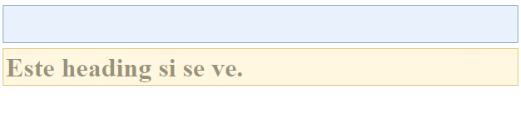
\includegraphics[width=10cm]{ss/visibility.png}
\end{figure}

Como podemos ver, esta propiedad esconde el elemento, pero mantiene su espacio en la página, a diferencia de la propiedad \textit{display none}.


\subsection{clear}

La propiedad \textbf{clear} de CSS ayuda a evitar que los elementos seguidos a uno que tiene la propiedad \textit{float} activa floten, es decir, \textbf{clear} evita que un elemento flote alrededor de otro. Los valores aceptados son:
\begin{itemize}
    \item \textbf{right}: evita flotar a la derecha de elementos con float.
    \item \textbf{left}: evita flotar a la izquierda de elementos con float.
    \item \textbf{both}: evita flotar en ambos lados de elementos con float.
    \item \textbf{none}: no evita flotar alrededor de elementos (valor predeterminado).
    \item \textbf{ihnerit}, \textbf{initial} y \textbf{unset}.
\end{itemize}

Dejamos un ejemplo y su resultado en la \textit{Figura \ref{fig: 30}}:
\begin{lstlisting}
estilos.css
    /* Los elementos flotan a la derecha de un elemento. */
    .floating {
        float: right;
    }
    /* Los elementos evitan flotar en ambos sentidos de un elemento. */
    .clearing {    
        clear: both;
    }
    /* Agrega borde sólido de 1 píxel a la imagen. */
    img {
        border-style: solid;
        border-width: 1px;
    }

prueba.html
    This paragraph is above the div element 
    and is not affected by the float right property. 
    <br/><br/>
    <div class="floating">
        <img src="http://www.sololearn.com/uploads/css_logo.png" height="300px"/>
    </div>
    This paragraph comes after the div element 
    and is affected by the float right property. 
    <div class="clearing">
        This paragraph is out of the floating group 
        and is not affected by the float right property.
    </div>
\end{lstlisting}
\begin{figure}[H]
    \centering
    \caption{Diferencia entre valores de propiedad \textit{clear}}
    \label{fig: 30}
    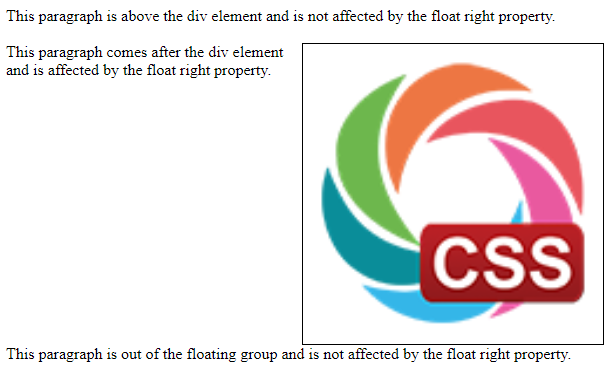
\includegraphics[width=12cm]{ss/clear.png}
\end{figure}


\subsection{overflow}

Recordemos que cada elemento HTML está contenido en una caja, cuando no establecemos el alto de la caja, este se ve ajustado automáticamente al contenido de la caja, sin embargo, si establecemos un alto y el contenido sobrepasa esta medida, se dice que ocurre un \textbf{desbordamiento} (\textit{overflow}), entonces, CSS tiene la propiedad \textbf{overflow}, que permite manejar el comportamiento del desbordamiento de contenido de los elementos. Los valores que acepta son:
\begin{itemize}
    \item \textbf{visible}: muestra completo el contenido desbordado del elemento (valor predeterminado).
    \item \textbf{scroll}: el contenido que sobresale es recortado y añade una barra de desplazamiento vertical y horizontal al elemento para ver el contenido que se desborda.
    \item \textbf{hidden}: el contenido que sobresale es recortado y no puede ser visto.
    \item \textbf{auto}: si el contenido es recortado, se añade una barra de desplazamiento vertical al elemento para ver el contenido que se desborda.
    \item \textbf{inherit}, \textbf{initial} y \textbf{unset}.
\end{itemize}

Dejamos un ejemplo y su resultado en la \textit{Figura \ref{fig: 31}}:
\begin{lstlisting}
estilos.css
    /* Pone los elementos uno al lado del otro. */
    .inline-block {
        display: inline-block;
    }
    /* Agrega un marge izquierdo de 10 píxeles. */
    p {
        margin-left: 10px;
    }
    /*
        Clases que reciben la propiedad "display" de su padre, se agrega un
        tamaño, borde y color para visualizar mejor el elemento, y se establece
        la propiedad "overflow".
    */
    .visible {
        display: inherit;
        width: 100px;
        height: 100px;
        border-style: solid;
        border-width: 1px;
        background-color: red;
        overflow: visible;
    }
    .hidden {
        display: inherit;
        width: 100px;
        height: 100px;
        border-style: solid;
        border-width: 1px;
        background-color: red;
        overflow: hidden;
    }
    .scroll {
        display: inherit;
        width: 100px;
        height: 100px;
        border-style: solid;
        border-width: 1px;
        background-color: red;
        overflow: scroll;
    }
    .auto {
        display: inherit;
        width: 100px;
        height: 100px;
        border-style: solid;
        border-width: 1px;
        background-color: red;
        overflow: auto;
    }

prueba.html
    <div class="inline-block">
        <p class="visible">Lorem ipsum dolor sit amet, consectetur adipiscing elit, sed do eiusmod tempor incididunt ut labore et dolore magna aliqua.</p>
        <p class="hidden">Lorem ipsum dolor sit amet, consectetur adipiscing elit, sed do eiusmod tempor incididunt ut labore et dolore magna aliqua.</p>
        <p class="scroll">Lorem ipsum dolor sit amet, consectetur adipiscing elit, sed do eiusmod tempor incididunt ut labore et dolore magna aliqua.</p>
        <p class="auto">Lorem ipsum dolor sit amet, consectetur adipiscing elit, sed do eiusmod tempor incididunt ut labore et dolore magna aliqua.</p>
    </div>
\end{lstlisting}
\begin{figure}[H]
    \centering
    \caption{Diferencia entre valores de propiedad \textit{overflow}}
    \label{fig: 31}
    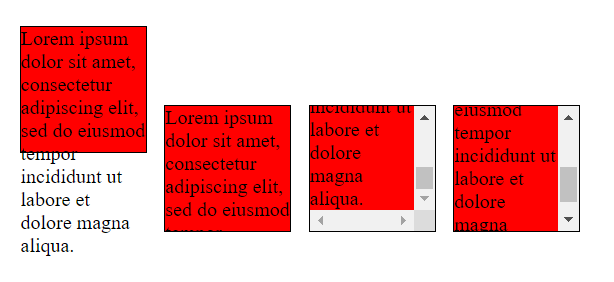
\includegraphics[width=11cm]{ss/overflow.png}
\end{figure}


\subsection{z-index}

Cuando una etiqueta se sobrepone en otra es debido a que, en el DOM y código HTML, la sobrepuesta va después de la que está por debajo, esto siempre ocurre, pero podemos cambiar el orden en el que se posicionan los elementos sobrepuestos. La propiedad \textbf{z-index} de CSS recibe como valores números enteros y da como resultado un ordenamiento de elementos sobrepuestos distinta. Veamos el siguiente código y su resultado (\textit{Figura \ref{fig: 32}}):
\begin{lstlisting}
estilos.css
    /* El primer contenedor tiene el "z-index" de 2. */
    .cont1 {
        position: fixed;
        top: 100px;
        left: 100px;
        width: 150px;
        height: 150px;
        background-color: red;
        /* "z-index" 2. */
        z-index: 2;
    }
    /* El segundo contenedor tiene el "z-index" de 1. */
    .cont2 {
        position: fixed;
        top: 180px;
        left: 180px;
        width: 150px;
        height: 150px;
        background-color: blue;
        color: white;
        /* "z-index" 1 */
        z-index: 1;
    }

prueba.html
    <div class="cont1">
        <p>Contenedor 1</p>
    </div>
    <div class="cont2">
        <p>Contenedor 2</p>
    </div>
\end{lstlisting}
\begin{figure}[H]
    \centering
    \caption{Funcionamiento de la propiedad \textit{z-index}}
    \label{fig: 32}
    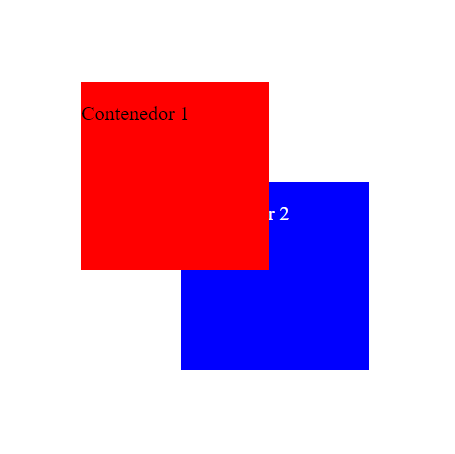
\includegraphics[width=7cm]{ss/z-index.png}
\end{figure}

Como vemos, el primer div con la clase "cont1" aparece, después, el siguiente div con la clase "cont2" aparece, ambos con la propiedad \textit{position} "fixed", el segundo div se sobrepone al primero por defecto, sin embargo, el estilo CSS le da a la clase "cont1" el valor 2 de \textit{z-index} y el valor 1 a la clase "cont2", por lo que "cont1" se sobrepone. No olvidar que la propiedad \textit{z-index} solamente funciona con elementos con la propiedad \textit{position} y el valor \textit{absolute}, \textit{relative} y \textit{fixed}.

\section{CSS3}

CSS3 es la versión más reciente de CSS, compatible con versiones anteriores del mismo, las características nuevas más significantes son el poder aplicar un radio e imagen a los bordes de elementos, varios fondos, animaciones y efectos.


\subsection{Prefijos del proveedor o buscador}

Los \textbf{prefijos del proveedor} (\textbf{o del buscador}) son instrucciones utilizadas para aplicar una propiedad a un buscador que no soporta dicha propiedad, por ejemplo, puede que Safari no soporte la propiedad \textit{border-radious}, por lo que hay que establecer el prefijo de Safari, seguido de la propiedad que deseamos utilizar en el sitio web, con esto, ya podremos trabajar con el radio de bordes de elementos. Los prefijos de algunos buscadores son:
\begin{itemize}
    \item \textbf{-webkit-}: prefijo para Safari, Chrome y buscadores que utilizan el motor \textit{Webkit} (iOS y Android).
    \item \textbf{-moz-}: prefijo para Firefox y buscadores que utilizan el motor de búsqueda de este.
    \item \textbf{-o-}: prefijo para Opera.
    \item \textbf{-ms-}: prefijo para Internet Explorer y Edge.
\end{itemize}

La sintaxis es la siguiente:
\begin{center}
    \textit{
        -webkit-border-radious: 8px; \\
        -o-border-radious: 8px; \\
        -moz-border-radious: 8px; \\
        -ms-border-radious: 8px; \\
    }
\end{center}

\textit{Nota}: actualmente, muchos buscadores ya integran todas las propiedades y características de CSS3, sin embargo, es recomendable conocer estos prefijos para tener una noción de que algunas propiedades tal vez no estén disponibles en el buscador donde estamos desarrollando un proyecto.


\subsection{Esquinas redondeadas}

La propiedad \textbf{border-radius} de CSS permite redondear todas las esquinas de un elemento. Podemos asignar un radio distinto por cada esquina con las propiedades \textbf{border-top-left-radius, border-top-right-radius, border-bottom-right-radius, border-bottom-left-radius}; esta propiedad cuenta con un acceso directo, para evitar escribir todas las propiedades anteriormente mencionadas una por una, como vemos en el siguiente ejemplo y su resultado en la \textit{Figura \ref{fig: 33}}:
\begin{lstlisting}
estilos.css
    /* Redondea todas las esquinas del contenedor en una sola instrucción. */
    .todo-redondeado {
        display: inherit;
        background-color: green;
        color: white;
        padding: 50px;
        margin-bottom: 5px;
        border-radius: 20px;
    }
    /* Redondea algunas esquinas del contenedor en varias instrucciones. */
    .separado-redondeado {
        display: inherit;
        background-color: green;
        color: white;
        padding: 50px;
        margin-bottom: 5px;
        border-top-right-radius: 10px;
        border-bottom-left-radius: 15px;
    }
    /* Redondea todas las esquinas del contenedor en varias instrucciones. */
    .todo-sep-redo {
        display: inherit;
        background-color: green;
        color: white;
        padding: 50px;
        margin-bottom: 5px;
        border-radius: 5px 7px 9px 11px;
    }
    .redondeado {
        display: block;
    }

prueba.html
    <div class="redondeado">
        <div class="todo-redondeado"></div>
        <div class="separado-redondeado"></div>
        <div class="todo-sep-redo"></div>
    </div>
\end{lstlisting}
\begin{figure}[H]
    \centering
    \caption{Diferencia entre valores de propiedad \textit{border-radious}}
    \label{fig: 33}
    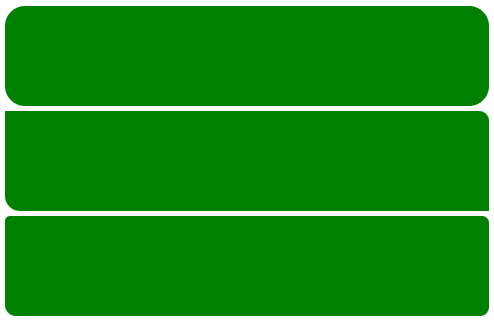
\includegraphics[width=8cm]{ss/border-radious.png}
\end{figure}

Como podemos ver, los valores que acepta esta propiedad son \textbf{Longitudes} (\%, px, pt, cm, em, etc.).


\subsection{Sombras}

La propiedad \textbf{box-shadow} de CSS permite agregar sombra a un elemento HTML. La forma en la que esta sombra es procesada por el buscador mediante los valores aceptados es la siguiente: el primer valor es el \textbf{largo de la sombra sobre el eje horizontal} del elemento, el segundo valor es el \textbf{largo de la sombra en el eje vertical} del elemento y el tercer valor es el \textbf{color de la sombra} (opcional). Además a estos valores, podemos agregar dos valores más: el \textbf{difuminado} y \textbf{propagación de la sombra} (\textit{blur} y \textit{spread}), como su nombre lo indica, modifican el difuminado de la sombra, y cómo esta se propaga alrededor del elemento. Veamos dos ejemplos, el primero sin difuminado ni propagación, el segundo si lo tiene, el resultado está en la \textit{Figura \ref{fig: 34}}:
\begin{lstlisting}
estilos.css
    /* Agrega sombra sin difuminar. */
    .bs1 {
        width: 300px;
        height: 100px;
        background-color: aquamarine;
        box-shadow: 10px 10px #152;
        margin-bottom: 20px;
    }
    /* Agrega sombra difuminada. */
    .bs2 {
        width: 300px;
        height: 100px;
        background-color:blue;
        box-shadow: 10px 10px 5px 5px #878787;
    }

pruebas.html
    <div class="redondeado">
        <div class="bs1"></div>
        <div class="bs2"></div>
    </div>
\end{lstlisting}
\begin{figure}[H]
    \centering
    \caption{Diferencia entre valores de propiedad \textit{box-shadow}}
    \label{fig: 34}
    
\includegraphics[width=8cm]{ss/box-shadow1.png}
\end{figure}

\textit{Nota}: asignar valores negativos a la propiedad ocasionará que la sombra se posicione en la esquina superior izquierda, no en la esquina inferior derecha.


\subsubsection{Técnicas para el sombreado}

Anteriormente vimos como crear una sombra para un elemento, pero solamente una, esta pudiendo tener su origen en dos ubicaciones distintas fuera del elemento, con la palabra reservada \textbf{inset} podemos crear una sombra dentro del elemento: esta palabra reservada va enseguida del nombre de la propiedad, y podemos asignarle valores como vimos en el tema anterior. Veamos la instrucción:
\begin{center}
    \textit{box-shadow: inset 10px 10px 5px \#888888;}
\end{center}

Esta instrucción creará una sombra interior ubicada en la esquina superior izquierda. Si queremos poner más sombras a un elemento, las podemos separar con una coma (,), como se ve en el siguiente ejemplo y resultado en la \textit{Figura \ref{fig: 35}}
\begin{lstlisting}
estilos.css
    /* Agrega una sombra interna sin difuminar. */
    .bs1 {
        width: 300px;
        height: 100px;
        background-color: aquamarine;
        box-shadow: inset 10px 10px #152;
        margin-bottom: 20px;
    }
    /* Agrega una sombra interna completa semi difuminada. */
    .bs2 {
        width: 300px;
        height: 100px;
        background-color:blue;
        box-shadow: 
        inset 10px 10px 5px 5px #878787,
        inset -10px -10px 5px 5px #878787;
        margin-bottom: 50px;
    }
    /* Agrega varias sombras externas completas difuminadas. */
    .bs3 {
        width: 300px;
        height: 100px;
        background-color:blue;
        box-shadow: 
        0 0 10px 4px #ff6347,
        0 0 10px 30px #ffdab9,
        30px 0 20px 30px #b0e0e6;
        margin-bottom: 20px;
        margin-left: 35px;
    }

prueba.html
    <div class="bs1"></div>
    <div class="bs2"></div>
    <div class="bs3"></div>
\end{lstlisting}
\begin{figure}[H]
    \centering
    \caption{Diferencia entre valores de propiedad \textit{box-shadow}}
    \label{fig: 35}
    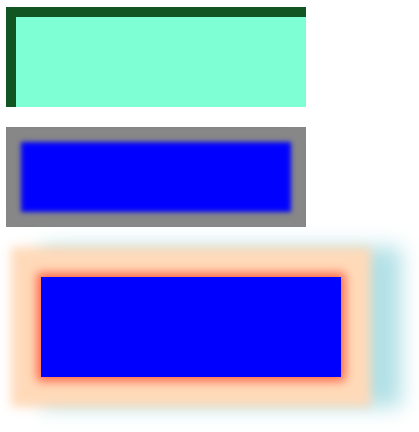
\includegraphics[width=8cm]{ss/box-shadow2.png}
\end{figure}

Como podemos ver, el primer rectángulo solo tiene una sombra interna, el segundo posee dos sombras internas, y el tercero posee tres sombras externas, una encima de otra, siguiendo el orden del código mostrado. Nótese que no existe una palabra reservada para sombras externas.


\subsubsection{Sombras en texto}

La propiedad \textbf{text-shadow} permite agregar una sombra al texto de un objeto o etiqueta HTML. Cuenta con cuatro valores: sombra horizontal, sombra vertical, difuminado y color; las sombras horizontal y vertical posiciona la sombra por debajo del texto en dichos ejes, podemos hacer que la sombra sea completamente definida o difuminada, y por último, podemos darle un color. Los primeros tres valores aceptan \textit{Longitudes} (\%, px, pt, cm, em, etc. También el valor \textit{none} para no asignar alguna sombra al texto), mientras que el último valor acepta valores de las distintas \textit{Herramientas de colores} con las que cuenta CSS.

Al igual que con \textit{box-shadow}, podemos crear varias sombras en el texto (inclusive negativas), veamos un ejemplo y su resultado en la \textit{Figura \ref{fig: 36}}:
\begin{lstlisting}
estilos.css
    /* Agrega una sombra. */
    .s1 {
        text-shadow: 3px 3px 2px #152;
        margin-bottom: 20px;
    }
    /* Agrega dos sombras. */
    .s2 {
        text-shadow: 
        10px 10px 5px #878787,
        -10px -10px 5px #900000;
        margin-bottom: 50px;
    }

prueba.html
    <p class="s1">Sombra 1</p>
    <p class="s2">Sombra 2</p>
\end{lstlisting}
\begin{figure}[H]
    \centering
    \caption{Diferencia entre valores de propiedad \textit{text-shadow}}
    \label{fig: 36}
    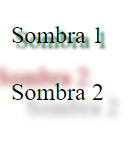
\includegraphics[width=3cm]{ss/text-shadow.png}
\end{figure}

Solo recuerde que las sombras se ven más realistas si:
\begin{itemize}
    \item una sombra cercana no está tan difuminada,
    \item una soma lejana si está más difuminada
\end{itemize}


\subsection{Transparencia}

Previo a CSS3, para lograr que un elemento tuviera transparencia, se utiliza la propiedad \textit{background-image} con una imagen en formato PNG, ahora, hay otros métodos para lograr este cometido. Con esta versión de CSS, se soporta ahora nombres de colores, hexadecimales, RGB y dos nuevas herramientas, que la \textit{Tabla \ref{tab: 4}} muestra:
\begin{table}[H]
    \centering
    \caption{Nuevas herramientas para colores en CSS3}
    \label{tab: 4}
    \begin{tabular}{m{3cm} m{8cm} m{4cm}}
        \hline
        \textbf{Herramienta} & \textbf{Definición} & \textbf{Ejemplo} \\
        \hline
        \parbox{3cm}{Colores RGBA}    & \parbox{8cm}{Extensión de los colores RGB con un valor \textbf{alfa}, el cual especifica la opacidad del color} & \parbox{4cm}{ rgba(204, 29, 29, 1.0); } \\
        \hline
        \parbox{3cm}{Colores HSL}     & \parbox{8cm}{Colores \textbf{Hue, Saturation, Lightness} (Matiz o color, Saturación, Luminosidad o claridad), es otra forma de expresar colores: el primero representa el color (los valores van de 0  360, donde 0 y 360 es rojo, 120 es verde y 240 es azul, en base a esto, se juega con estos valores para obtener el color deseado), el segundo la saturación (se mide en porcentajes, 100\% es el color completo y como tal) y el tercero la claridad del color (0\% es oscuro o negro, 100\% es blanco)} & \parbox{4cm}{ hsl(0, 10\%, 60\%); } \\
        \hline
        \parbox{3cm}{Colores HSLA}    & \parbox{8cm}{Extensión de los colores HSL con un valor \textbf{alfa}, el cual especifica la opacidad del color} & \parbox{4cm}{ hsla(147, 50\%,\\ 47\%, 0.5); } \\
        \hline
    \end{tabular}
\end{table}

Veamos el resultado de los ejemplos anteriores en la \textit{Figura \ref{fig: 37}}:
\begin{lstlisting}
estilos.css
    /* Establece color con RGBA y sin transparencia (1.0). */
    #rgba1 {
        width: 100px;
        height: 100px;
        background-color: rgba(204, 29, 29, 1.0);
        margin-bottom: 10px;
    }
    /* Establece color con RGBA y con transparencia de 0.1. */
    #rgba2 {
        width: 100px;
        height: 100px;
        background-color: rgba(161, 30, 30, 0.1);
        margin-bottom: 10px;
    }
    /* Establece color con HSL y con transparencia del 60%. */
    #hsl1 {
        width: 100px;
        height: 100px;
        background-color: hsl(0, 10%, 60%);
        margin-bottom: 10px;
    }
    /* Establece color con HSLA y con transparencia de 0.5. */
    #hsl2 {
        width: 100px;
        height: 100px;
        background-color: hsla(147, 50%, 47%, 0.5);
    }

prueba.html
    <div id="rgba1"></div>
    <div id="rgba2"></div>
    <div id="hsl1"></div>
    <div id="hsl2"></div>
\end{lstlisting}
\begin{figure}[H]
    \centering
    \caption{Uso de RGBA, HSL y HSLA}
    \label{fig: 37}
    
\includegraphics[height=9cm]{ss/rgba,hsl,hsla.png}
\end{figure}


\subsection{Pseudo clases}

Bien vimos que, para estilizar un elemento específico, le asignamos un Id o Clase, y dicha Clase o Id, se le aplican instrucciones CSS. En caso de que se tengan múltiples etiquetas dentro de otra, cada una de ellas debería tener una Clase o Id para ser modificadas por separado.

Es aquí donde entran las \textbf{Pseudo clases}, estas permiten modificar un elemento sin tener que asignarle una Clase o Id ni utilizar JavaScript. Existen muchas Pseudo clases, para estos apuntes, hablaremos de \textit{:first-child} y \textit{:last-child}:
\begin{itemize}
    \item \textbf{:first-child}: aplica un estilo al primer elemento dentro de otro.
    \item \textbf{:last-child}: aplica un estilo al último elemento dentro de otro.
\end{itemize}

Veamos un ejemplo y su resultado en la \textit{Figura \ref{fig: 38}}:
\begin{lstlisting}
estilos.css
    /* Clase padre con color de texto rojo. */
    .pseudo {
    color: red;
    }
    /* Cambia el color de texto del primer hijo de la clase padre. */
    .pseudo p:first-child {
        color: blue;
    }
    /* Cambia el color de texto del último hijo de la clase padre. */
    .pseudo p:last-child {
        color: violet;
    }

prueba.html
    <div class="pseudo">
        <p>Este es el primer párrafo.</p>
        <p>Este es el segundo párrafo.</p>
        <p>Este es el tercer párrafo.</p>
        <p>Este es el cuarto párrafo.</p>
        <p>Este es el quinto párrafo.</p>
        <p>Este es el sexto párrafo.</p>
    </div>
\end{lstlisting}
\begin{figure}[H]
    \centering
    \caption{Uso de las Pseudo clases}
    \label{fig: 38}
    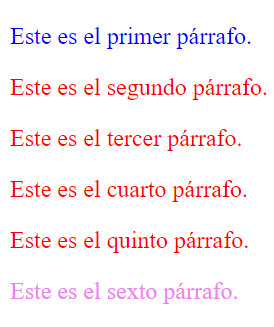
\includegraphics[height=5cm]{ss/pseudo-clases.png}
\end{figure}

Estas dos Pseudo clases son de las más utilizadas, pero existen más, te invito a investigar qué utilidad tienen el resto de Pseudo clases disponibles.


\subsection{Pseudo elementos}

Otra gran utilidad de estas Pseudo herramientas disponibles en CSS son los \textbf{Pseudo elementos}, estos permiten estilizar una parte o elemento de una etiqueta HTML. Las Pseudo clases utilizan los \textit{dos puntos} (:), los Pseudo elementos utilizan \textit{doble dos puntos} (::) para ser trabajados. Los cinco Pseudo elementos más utilizados son:
\begin{itemize}
    \item \textbf{::first-line}: selecciona la primer línea de un texto en una etiqueta.
    \item \textbf{::first-letter}: selecciona la primer letra de un texto o palabra en una etiqueta.
    \item \textbf{::selection}: toma el texto seleccionado de una etiqueta por el usuario
    \item \textbf{::before}: inserta un contenido antes de una etiqueta.
    \item \textbf{::after}: inserta un contenido después de una etiqueta.
\end{itemize}

Algunos de estos Pseudo elementos no están disponibles en ciertos navegadores, por lo que tendrá que acudir a los \textbf{prefijos de buscadores}. Veamos un ejemplo de estos Pseudo elementos y su resultado en la \textit{Figura \ref{fig: 39}}:
\begin{lstlisting}
estilos.css
    /* Cambia el color de la primer letra. */
    p::first-letter {
        color: blue;
    }
    /* Cambia el color de la primer línea del texto. */
    p::first-line {
        color: red;
    }
    /* Cambia el color del texto seleccionado. */
    p::selection {
        background-color: green;
        color:white;
    }
    /* Agrega algo antes de un elemento. */
    p::before {
        content: url(bola.png);
    }
    /* Agrega algo después de un elemento. */
    p::after {
        content: url(bola.png);
    }

prueba.html
    <div class="pseudo">
        <p>Lorem ipsum dolor sit amet consectetur adipisicing elit. Assumenda distinctio ullam delectus porro odit sequi aperiam, amet commodi molestias beatae veniam obcaecati similique sint nulla, consequuntur veritatis, magni autem est.</p>
        <p>Lorem ipsum dolor sit amet consectetur adipisicing elit. Assumenda distinctio ullam delectus porro odit sequi aperiam, amet commodi molestias beatae veniam obcaecati similique sint nulla, consequuntur veritatis, magni autem est.</p>
        <p>Lorem ipsum dolor sit amet consectetur adipisicing elit. Assumenda distinctio ullam delectus porro odit sequi aperiam, amet commodi molestias beatae veniam obcaecati similique sint nulla, consequuntur veritatis, magni autem est.</p>
        <p>Lorem ipsum dolor sit amet consectetur adipisicing elit. Assumenda distinctio ullam delectus porro odit sequi aperiam, amet commodi molestias beatae veniam obcaecati similique sint nulla, consequuntur veritatis, magni autem est.</p>
        <p>Lorem ipsum dolor sit amet consectetur adipisicing elit. Assumenda distinctio ullam delectus porro odit sequi aperiam, amet commodi molestias beatae veniam obcaecati similique sint nulla, consequuntur veritatis, magni autem est.</p>
    </div>
\end{lstlisting}
\begin{figure}[H]
    \centering
    \caption{Uso de los Pseudo elementos}
    \label{fig: 39}
    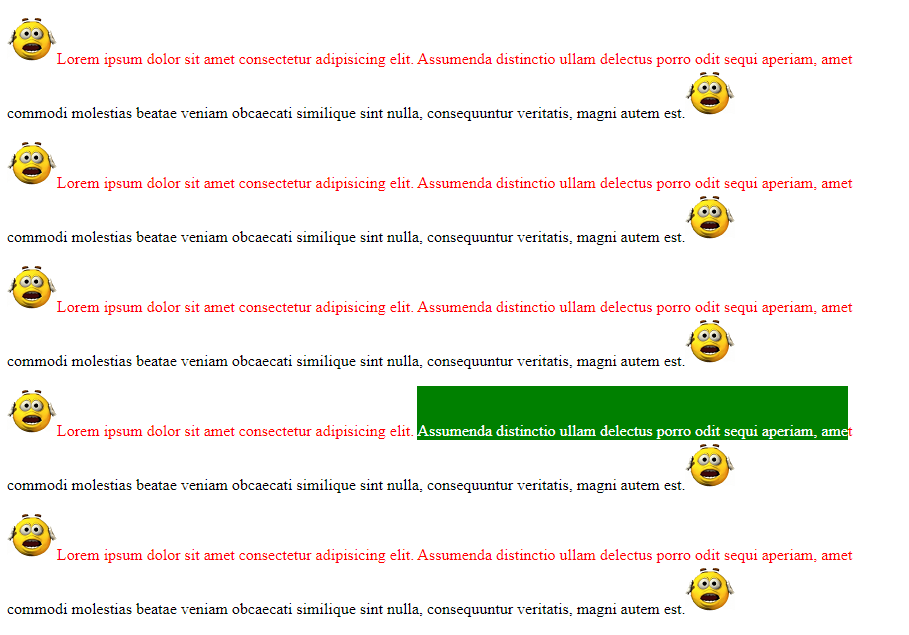
\includegraphics[width=12cm]{ss/pseudo-elementos.png}
\end{figure}

En el caso de \textit{first-letter} esta se ve sobre escrita por \textit{first-line}, por lo cual no se aprecia en la figura anterior. Al igual que con las Pseudo clases, se le invita a investigar más Pseudo elementos existentes.


\subsection{word-wrap}
\
La propiedad \textbf{word-wrap} de CSS permite establecer si una palabra da un salto de línea cuando topa con el límite de su etiqueta o contenedor; los valores permitidos son:
\begin{itemize}
    \item \textbf{normal}: el texto mantiene su largo.
    \item \textbf{break-word}: el texto da un salto de línea.
    \item \textbf{inherit}, \textbf{initial} y \textbf{unset}.
\end{itemize}

Veamos un ejemplo claro de esta propiedad y su resultado en la \textit{Figura \ref{fig: 40}}:
\begin{lstlisting}
estilos.css
    /* Clase que no da salto de línea. */
    .wwn {
        width: 200px;
        height: 100px;
        border: 2px solid black;
        word-wrap: normal;
    }
    /* Clase que no da salto de línea. */
    .wwww {
        width: 200px;
        height: 100px;
        border: 2px solid black;
        word-wrap: break-word;
    }

prueba.html
    <p class="wwn">Esta caja tiene una palabra muy larga: njfsadfnjiaifiafiaisiajfisjadifisadnfsiadfnjisdjfjiasdfjisadfidanjinj</p>
    <p class="wwww">Esta caja tiene una palabra muy larga: njfsadfnjiaifiafiaisiajfisjadifisadnfsiadfnjisdjfjiasdfjisadfidanjinj</p>
\end{lstlisting}
\begin{figure}[H]
    \centering
    \caption{Diferencia entre valores de propiedad \textit{word-wrap}}
    \label{fig: 40}
    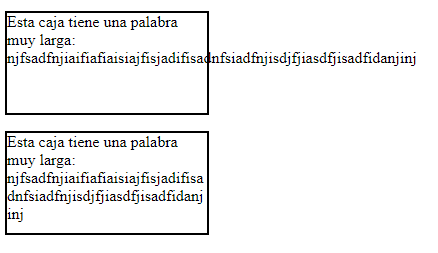
\includegraphics[width=10cm]{ss/word-wrap.png}
\end{figure}


\subsection{@font-face}

La regla \textbf{@font-face} permite descargar u obtener una fuente o tipo de letra de un servidor y establecerla en todo nuestro sitio web, de esta manera, las fuentes disponibles en el sitio ya no están limitadas en las que están instaladas en la máquina del usuario que accede al sitio.

Esta regla trabaja con los formatos \textbf{Embedded OpenType} (eot), \textbf{True Type Fonts} (ttf) y \textbf{OpenType Fonts} (otf), los siguientes navegadores aceptan los formatos mencionados:
\begin{itemize}
    \item Firefox, Safari, Chrome y Opera: .ttf y .otf.
    \item Internet Explorer: .eot
\end{itemize}

Para utilizar esta regla, debe escribir el nombre de la regla (@font-face), abrir llaves, darle un nombre a la fuente, la ruta donde está almacenada la fuente y alguna personalización extra, como se ve a continuación:
\begin{lstlisting}
estilos.css
    /* Define dos reglas iguales pero con distinto estilo. */
    @font-face {
      font-family: Delicious; 
      src: url('Delicious-Roman.otf'); 
    } 
    @font-face { 
      font-family: Delicious; 
      font-weight: bold; 
      src: url('Delicious-Bold.otf'); 
    }
    /* Asigna las reglas a las etiquetas "h1". */
    h1 {
       font-family: Delicious, sans-serif; 
    }

prueba.html
    <h1>Hola mundo</h1>
\end{lstlisting}

En caso de que queramos que todo el sitio tenga la nueva fuente, en vez de asignarla a la etiqueta "h1", se la asignamos a "body."

Las fuentes más utilizadas actualmente son las de Google, esto debido a que es por este buscador que los usuarios se conectan a Internet y realizan sus búsquedas, por lo que es bueno utilizar dichas fuentes para cargar nuestro sitio web, puede ver todas las fuentes disponibles en este \href{https://fonts.google.com/}{enlace} (aunque tiene una distinta implementación).

Puede buscar fuentes con los formatos anteriormente mencionados en Internet y aplicarlas al sitio web, como se ve en el ejemplo siguiente y su resultado en la \textit{Figura \ref{fig: 41}}:
\begin{lstlisting}
estilos.css
    /* Asigna la fuente importada a las etiquetas "h1". */
    h1 {
        font-family: 'Open Sans', sans-serif;
    }
    
prueba.html
    <h1>Hola mundo</h1>
\end{lstlisting}
\begin{figure}[H]
    \centering
    \caption{Uso de la regla \textit{@font-face}}
    \label{fig: 41}
    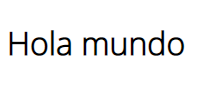
\includegraphics[width=3cm]{ss/font-face.png}
\end{figure}

\section{Degradados}

CSS3 permite que se establezca una transición suave o lisa entre dos o más colores. Estos tipos de transiciones o degradados están categorizados en dos tipos: \textbf{lineal} y \textbf{radial}.


\subsection{Degradado lineal}

Para crear un degradado lineal, se utiliza el método \textbf{linear-gradient()}, se deben establecer dos \textbf{escalas de colores}, estas dos escalas de colores renderizarán la transición suave; a estos degradados se le puede establecer un punto de origen y una dirección (o un ángulo). Veamos un ejemplo y su resultado en la \textit{Figura \ref{fig: 42}}:
\begin{lstlisting}
estilos.css
    div {
        width: 300px; 
        height: 100px;
        color: gray;  
        /* Degradado lineal blanco y negro. */
        background: -moz-linear-gradient(black, white);
        font-size: larger;
    }

prueba.html
    <div>
        Hola mundo
    </div>
\end{lstlisting}
\begin{figure}[H]
    \centering
    \caption{Utilizando el degradado lineal simple}
    \label{fig: 42}
    
\includegraphics[width=7cm]{ss/linear-gradient-1.png}
\end{figure}


\subsubsection{Prefijos, múltiples escalas y presencia en el degradado}

El ejemplo anterior tiene el \textbf{prefijo del buscador} de Mozilla Firefox, para que este degradado funcione dentro de dicho buscador, pero puede ser agregado, removido o cambiado por otro prefijo en caso de ser requerido. Para el caso de estos apuntes y prácticas, los degradados fueron creados con el buscador \textbf{Microsoft Edge}, el cual no requirió de un prefijo.

En el caso anterior, utilizamos solamente dos escalas de colores con sus respectivas palabras reservadas, pero podemos agregar más de dos, simplemente se agregan separando las escalas por comas, de igual manera, podemos tener, por ejemplo, cinco colores, pero queremos que el cuarto sea el que aparezca más en el degradado, podemos conseguir esto agregando una \textbf{Longitud} (\%, px, pt, cm, em, etc.), como se ve a continuación (\textit{Figura \ref{fig: 43}}):
\begin{lstlisting}
estilos.css
    div {
        width: 500px; 
        height: 300px;
        color: white;
        /* Degradado lineal blanco, negro, rojo y azul al 50% y añade verde. */
        background: linear-gradient(black, white, red, blue 50%, green);
        font-size: larger;
    }

prueba.html
    <div>
        Hola mundo
    </div>
\end{lstlisting}
\begin{figure}[H]
    \centering
    \caption{Utilizando el degradado lineal múltiple}
    \label{fig: 43}
    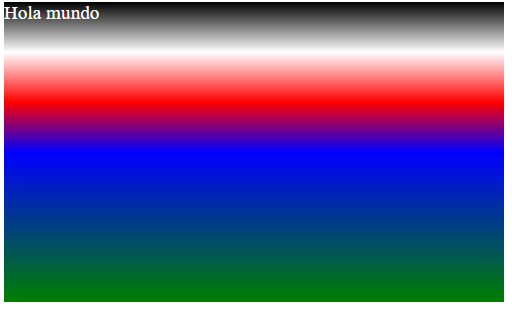
\includegraphics[width=7cm]{ss/linear-gradient-2.png}
\end{figure}

Como vemos, el cuarto color (azul) es el que tiene más presencia, debido a que le asignamos que tuviera una presencia del 50\%.


\subsubsection{Dirección o ángulo del degradado}
\
Podemos lograr que el degradado comience desde distintas \textbf{ubicaciones} del elemento: izquierda, derecha, arriba o abajo, las palabras reservadas \textbf{left}, \textbf{right}, \textbf{top} y \textbf{bottom} respectivamente (también podemos utilizar las esquinas del elemento, por ejemplo, la esquina superior izquierda, que sería \textbf{top left}). 

Considere que, si no utiliza los \textit{prefijos de un buscador}, debe agregar la palabra reservada \textbf{to} previo al valor de dirección predeterminado escogido, si sí va a utilizar un prefijo, no agregue \textbf{to}.
\begin{center}
    \textit{
        // Sin prefijo: \\
        background: linear-gradient(to left, red, blue); \\
        // Con prefijo: \\
        background: -moz-linear-gradient(left, red, blue);
    }
\end{center}

Por otro lado, una alternativa a estas palabras predefinidas son los ángulos, que puede ir desde 0 a 360 grados, si escribimos el valor \textit{0deg}, creará un degradado de izquierda a derecha, mientras que si escribimos el valor \textit{90deg}, creará un degradado de abajo a arriba, experimente con los distintos valores para crear un degradado de su agrado.

Veamos como se ven estas dos formas de dirección en el siguiente ejemplo y su resultado en la \textit{Figura \ref{fig: 44}}:
\begin{lstlisting}
estilos.css
    #dir {
        width: 500px; 
        height: 300px;
        color: white;  
        /* Dirección de degradado con palabras reservadas. */
        background: linear-gradient(to bottom left, red, blue, green);
        font-size: larger;
    }
    
    #ang {
        width: 500px; 
        height: 300px;
        color: white;
        /* Dirección de degradado con ángulos. */
        background: linear-gradient(56deg, pink, purple, orange);
        font-size: larger;
    }

prueba.html
    <div id="dir">
        Con palabras predefinidas
    </div>
    <div id="ang">
        Con ángulos
    </div>
\end{lstlisting}
\begin{figure}[H]
    \centering
    \caption{Utilizando el degradado lineal con dirección}
    \label{fig: 44}
    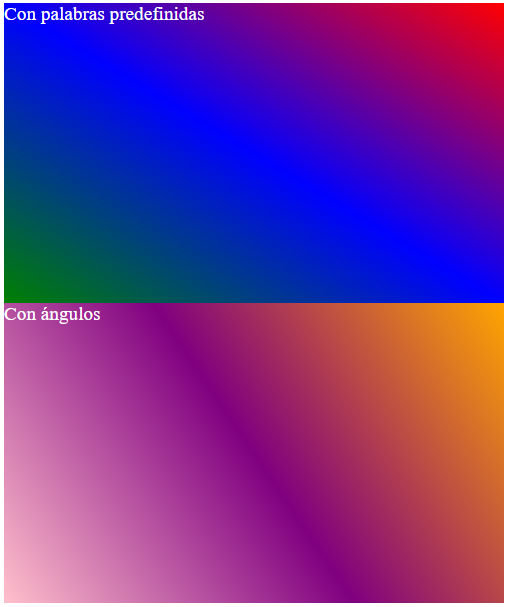
\includegraphics[width=7cm]{ss/linear-gradient-3.png}
\end{figure}


\subsubsection{Repetir el degradado}

Puede repetir un degradado en un mismo elemento con el método \textbf{repeating-linear-gradiant()}, añadiendo una \textbf{Longitud} (\%, px, pt, cm, em, etc.) después de la escala de color. Esta propiedad también acepta las direcciones de degradado. Veamos un ejemplo y su resultado en la \textit{Figura \ref{fig: 45}}:
\begin{lstlisting}
estilos.css
    div {
        width: 500px; 
        height: 300px;
        color: white;
        /* Repite el degradado azul y verde a un 30%. */
        background: repeating-linear-gradient(blue, green 30%);
        font-size: larger;
    }
    
prueba.html
    <div>
        Hola mundo
    </div>
\end{lstlisting}
\begin{figure}[H]
    \centering
    \caption{Repitiendo un degradado lineal}
    \label{fig: 45}
    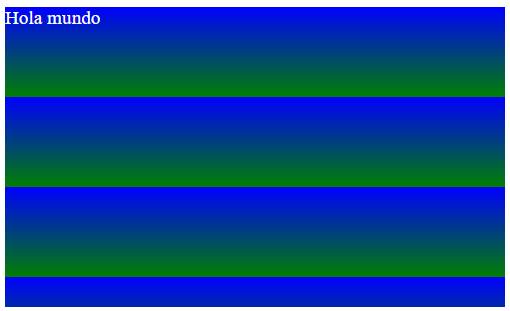
\includegraphics[width=7cm]{ss/linear-gradient-4.png}
\end{figure}

Tomamos el 30\% del tamaño del elemento y metemos ahí al degradado, así con el siguiente 30\% y así sucesivamente.


\subsection{Degradado radial}

La otra manera de definir un degradado a un elemento es por medio del método \textbf{radial-gradient()}, el cual tiene la siguiente sintaxis:
\begin{center}
    \textit{radial-gradient(forma tamaño \textbf{at} posición, escalas de colores);}
\end{center}

Donde:
\begin{itemize}
    \item \textbf{forma}: indica la forma del degradado. Los valores aceptados son \textit{ellipse} (por defecto) y \textit{circle}.
    \item \textbf{tamaño}: indica el tamaño del degradado. Los valores aceptados son \textit{farthest-corner} (por defecto), \textit{closest-side}, \textit{closest-corner} y \textit{farthest-side}.
    \item \textbf{posición}: indica donde comienza el degradado. Se pueden utilizar palabras reservadas (top, bottom, left, right o una combinación de estas) o Unidades de valores, la unidad más común a utilizar es el porcentaje (\%), por ejemplo, 0\%, 0\% hace que el degradado comience en la esquina superior izquierda; 50\%, 50\% hace que comience a la mitad. El valor por defecto es centrado (si es que este parámetro es omitido).
    \item \textbf{escala de colores}: indica los colores del degradado; se pueden poner más de dos, separados por comas, además, se puede repetir los colores como con el estilo de degradado anterior.
\end{itemize}

Mostramos a continuación algunos ejemplos en la \textit{Figura \ref{fig: 46}}:
\begin{lstlisting}
estilos.css
    /* Despliega los contenedores uno al lado del otro. */
    .cont {
        display: inline-block;
    }
    /* Crea contenedores de tamaño fijo, con degradado radial de tres colores y forma de elipse. */
    .rad1 {
        display: inherit;
        width: 300px;
        height: 200px;
        background-image: radial-gradient(red, orange, yellow);
    }
    /* Degradado con repetición de colores y forma circular. */
    .rad2 {
        display: inherit;
        width: 300px;
        height: 200px;
        background-image: radial-gradient(circle, pink 10px, purple 91px);
    }
    /* Degradado de cierto tamaño y posición con forma circular. */
    .rad3 {
        display: inherit;
        width: 300px;
        height: 200px;
        background-image: radial-gradient(circle farthest-side at 30% 70%, blue, green, aqua);
    }

prueba.html
    <div class="cont">
        <div class="rad1"></div>
        <div class="rad2"></div>
        <div class="rad3"></div>
    </div>
\end{lstlisting}
\begin{figure}[H]
    \centering
    \caption{Utilizando el degradado radial}
    \label{fig: 46}
    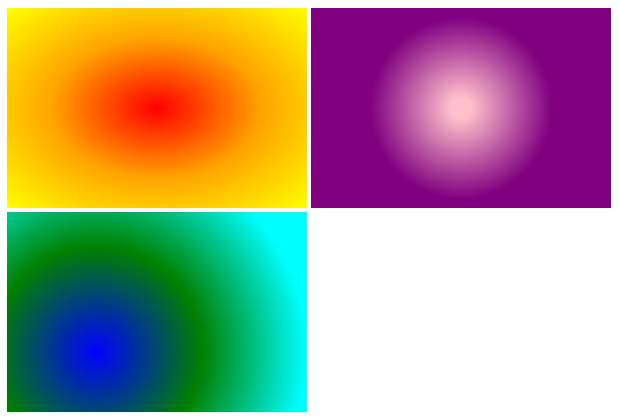
\includegraphics[width=10cm]{ss/radial-gradient.png}
\end{figure}

Como se puede apreciar, se combina la sintaxis de esta función en los tres ejemplos anteriores.



\section{Fondos}


\subsection{background-size}

La propiedad \textbf{background-size} de CSS permite cambiar el tamaño del fondo de un elemento mediante el escalado de la imagen. La mayoría de buscadores ya soportan esta propiedad, por lo que no es necesario agregar un \textit{Prefijo del buscador}. Esta propiedad acepta Unidades de valores o tres palabras reservadas:
\begin{itemize}
    \item \textbf{auto}: por defecto, establece el tamaño de la imagen del fondo tal cual es.
    \item \textbf{contains}: hace que el alto de la imagen del fondo y el alto del elemento HTML sean el mismo. Si el ancho de la imagen de fondo es menor al del elemento, repite la imagen, si no lo es, se ajusta.
    \item \textbf{cover}:  Hace que el ancho de la imagen del fondo y el alto del elemento HTML sean el mismo. Si el alto de la imagen de fondo es es menor al del elemento, se ajusta, si no lo es, se recorta la imagen con respecto al tamaño del elemento.
    \item \textbf{Longitudes} (\%, px, pt, cm, em, etc.).
    \item \textbf{inherit}, \textbf{initial} y \textbf{unset}.
\end{itemize}

La diferencia entre \textit{contains} y \textit{cover} se puede ver a continuación en la \textit{Figura \ref{fig: 47}}:
\begin{lstlisting}
estilos.css
    /* Despliega los contenedores uno al lado del otro. */
    .cont {
        display: inline-block;
    }
    .contains {
        display: inherit;
        /* Tamaño de la clase para ejemplificar la propiedad "background-size". */
        width: 400px;
        height: 250px;
        background-image: url(gato.png);
        background-size: contain;
    }
    .cover {
        display: inherit;
        width: 400px;
        height: 250px;
        background-image: url(gato.png);
        background-size: cover;
    }

prueba.html
    <div class="cont">
        <div class="contains"></div>
        <div class="cover"></div>
    </div>
\end{lstlisting}
\begin{figure}[H]
    \centering
    \caption{Diferencia entre los valores \textit{contains} y \textit{cover}}
    \label{fig: 47}
    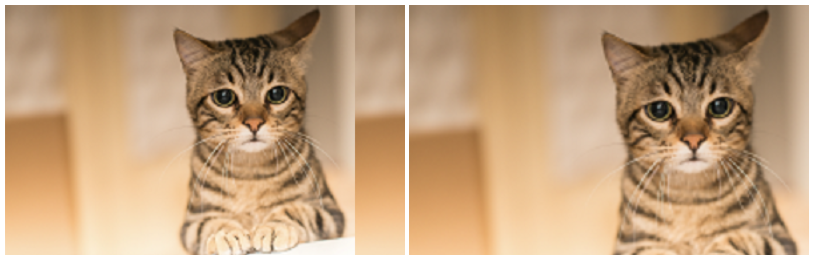
\includegraphics[width=12cm]{ss/background-size.png}
\end{figure}

Como vemos, el ancho del primer elemento es mayor a la imagen de fondo que se le establece, por lo que esta imagen se repite; para el segundo contenedor, el ancho de la imagen y el elemento se ajusta, pero el alto de la imagen de fondo es mayor al alto de su elemento, por lo que la imagen se termina cortando y no mostrándose completamente, esta es la principal diferencia entre ambos valores de la propiedad.


\subsection{background-clip}

La propiedad \textbf{background-clip} de CSS delimita hasta donde se colorea o se aplica una imagen al fondo de un elemento. Los valores aceptados son:
\begin{itemize}
    \item \textbf{border-box}: valor por defecto, colorea o aplica una imagen a un fondo por completo, incluyendo el borde del elemento.
    \item \textbf{padding-box}: colorea o aplica una imagen a un fondo, descartando el padding del elemento.
    \item \textbf{content-box}: colorea o aplica una imagen a un fondo por completo, excluyendo el borde del elemento.
    \item \textbf{initial}, \textbf{unset} y \textbf{inherit}.
\end{itemize}

La diferencia de estos valores se aprecia en la \textit{Figura \ref{fig: 48}}
\begin{lstlisting}
estilos.css
    /* Establece un tipo de borde, padding, color de fondo iguales
    para cada div y la propiedad "background-clip" distinta. */
    #first {
        border: 2px dotted black;
        padding: 20px;
        background: LightBlue;
        background-clip: padding-box;
    }
    #second {
        border: 2px dotted black;
        padding: 20px;
        background: LightBlue;
        background-clip: content-box;
    }
    #third {
        border: 2px dotted black;
        padding: 20px;
        background: LightBlue;
        background-clip: border-box;
    }

prueba.html
    <div id="first">
        <p>background-clip: padding-box</p>
    </div>
    <div id="second">
        <p>background-clip: content-box</p>
    </div>
    <div id="third">
        <p>background-clip: content-box</p>
    </div>
\end{lstlisting}
\begin{figure}[H]
    \centering
    \caption{Diferencia entre los valores \textit{border-box}, \textit{padding-box} y \textit{content-box}}
    \label{fig: 48}
    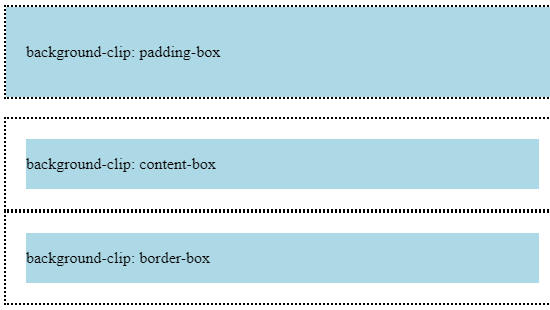
\includegraphics[width=8cm]{ss/background-clip.png}
\end{figure}


\subsection{Bordes transparentes}

Un borde transparente para un elemento se consigue combinando la propiedad \textit{background-clip} y el \textit{RGBA} (\textit{Figura \ref{fig: 49}}):
\begin{lstlisting}
estilos.css
    div {
        /* Borde de 20px de grosor negro y con transparencia de 0.1. */
        border: 20px solid rgba(0, 0, 0, 0.1);
        /* Colorea el borde. */
        background-clip: padding-box; 
        /* Posiciona el div. */
        position:absolute;
        top:50px;
        left:50px;
        width:200px;
        /* Fondo blanco. */
        background-color:white;
    }

prueba.html
    <div>In the screenshot, we set the background-clip to padding-box. The white background ends before the border and the transparency lays over the content</div>

    Some text Some text Some text Some text Some text Some text Some text Some text Some text Some text Some text Some text Some text Some text Some text Some text Some text Some text Some text Some text Some text Some text Some text Some text Some text Some text Some text Some text Some text Some text Some text Some text Some text Some text Some text Some text Some text Some text Some text Some text Some text Some text Some text Some text Some text Some text Some text Some text Some text Some text Some text Some text Some text Some text Some text Some text Some text Some text Some text Some text Some text Some text Some text Some text
\end{lstlisting}
\begin{figure}[H]
    \centering
    \caption{Consiguiendo un borde transparente}
    \label{fig: 49}
    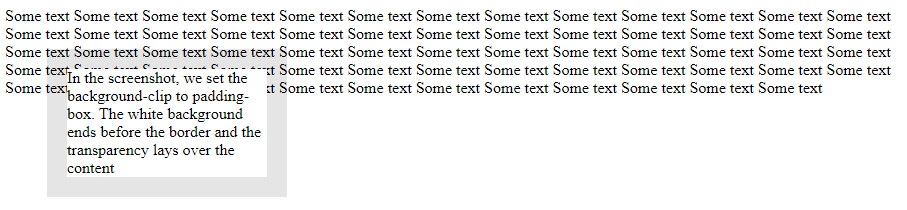
\includegraphics[width=12cm]{ss/borde-transparente.png}
\end{figure}


\subsection{Varias imágenes de fondo}

Podemos poner múltiples fondos a un elemento creando una lista de elementos separados por comas, recordemos que existe el método \textbf{url()}, la cual permite que pongamos un fondo de Internet o del directorio donde estemos trabajando. Las imágenes se van poniendo de \textbf{arriba a abajo}, por lo que la primera irá hasta arriba y la última hasta abajo, como en el siguiente ejemplo (\textit{Figura \ref{fig: 50}}):
\begin{lstlisting}
estilos.css
    div {
        border: 1px solid black;
        width: 400px;
        height: 300px;
        /* Varias imágenes separadas por comas (,). */
        background-image: url("bola.png"), url("gato.png");
        background-position: top, bottom;
        background-repeat: no-repeat;
    }

prueba.html
    <div></div>
\end{lstlisting}
\begin{figure}[H]
    \centering
    \caption{Múltiples fondos}
    \label{fig: 50}
    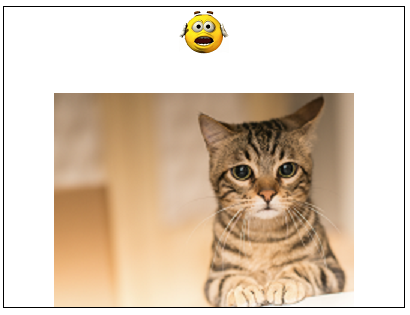
\includegraphics[width=7cm]{ss/multiples-bordes.png}
\end{figure}


\subsubsection{background-position}

Como pudimos ver en el ejemplo anterior, nos saltamos la regla de que los múltiples fondos van de arriba a abajo, los posicionamos distinto mediante una lista separada por comas, esto gracias a la propiedad \textbf{background-position}, esta nos permite establecer la posición de inicio de una imagen de fondo. Los valores aceptados son:
\begin{itemize}
    \item \textbf{left top, left center y left bottom}: comenzando desde la izquierda a arriba, en medio o abajo respectivamente.
    \item \textbf{right top, right center y right bottom}: comenzando desde la derecha a arriba, en medio o abajo respectivamente
    \item \textbf{center top, center center y center bottom}: comenzando del centro a arriba, en medio o abajo respectivamente.
    \item \textbf{Longitudes} (\%, px, pt, cm, em, etc.).
    \item \textbf{initial}, \textbf{unset} y \textbf{inherit}.
\end{itemize}

Los valores con palabra reservada se pueden mezclar, es por eso que los pusimos directamente como \textit{left top}, \textit{right center} o \textit{center bottom}, pero también puede utilizarlos como palabra sola (\textit{top}, \textit{left}, \textit{right} y \textbf{bottom}).

También puede utilizar la propiedad recortada \textit{background} para establecer la imagen, su posición y si se repite o  no:
\begin{center}
    \textit{background: url([imagen]) [posición] [repetir]}
\end{center}


\subsection{opacity}

La propiedad \textbf{opacity} permite volver transparente una imagen de manera sencilla, ya que su valor tope es 1 (opaco) y su valor mínimo es 0 (completamente transparente), por lo que debe establecer un valor decimal entre ambos topes, como se ve en la \textit{Figura \ref{fig: 51}}:
\begin{lstlisting}
estilos.css
    /* Imagen con opacidad de 0.5. */
    #img1 {
        width: 400px;
        height: 400px;
        background-image: url("gato.png");
        background-repeat: no-repeat;
        opacity: 0.5;
    }
    #img2 {
        /* Imagen con opacidad de 0.2. */
        width: 400px;
        height: 400px;
        background-image: url("gato.png");
        background-repeat: no-repeat;
        opacity: 0.2;
    }

prueba.html
    <div id="img1"></div>
    <div id="img2"></div>
\end{lstlisting}
\begin{figure}[H]
    \centering
    \caption{Transparencia de imágenes}
    \label{fig: 51}
    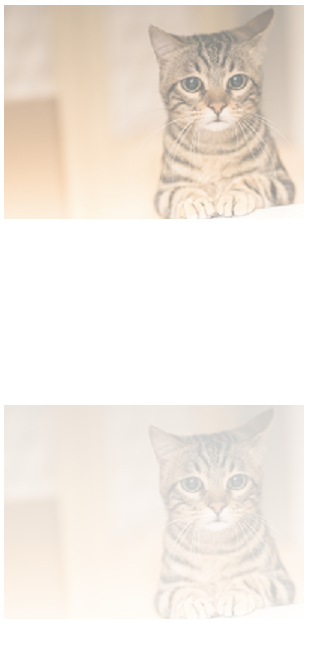
\includegraphics[width=7cm]{ss/opacity.png}
\end{figure}

\section{Transiciones}

Las \textbf{transiciones} nos permiten pasar de un valor de propiedad a otro dada una duración. La sintaxis básica es la siguiente:
\begin{center}
    \textit{transition: propiedad duración}
\end{center}

Donde:
\begin{itemize}
    \item \textbf{propiedad}: especifica la propiedad que tendrá la transición.
    \item \textbf{duración}: especifica el tiempo de duración de la transición.
\end{itemize}

La propiedad \textit{transition} de CSS se le debe asignar al elemento que se desea que tenga una animación, pero de momento todavía no hace nada; en caso de que se omita alguno de los dos valores básicos anteriores, la animación no funcionará. Para hacer que la animación se haga, se debe establecer un nuevo valor para el valor \textit{propiedad} de \textit{transition}, esto debe ser fuera del elemento a animar, como por ejemplo, si hacemos que el puntero del mouse se ponga encima del elemento, cambie de tamaño:
\begin{lstlisting}
    div {
        /* Valor inicial de la propiedad a animar. */
        width: 100px;
        height: 100px;
        background: red;
        /* Establece la propiedad a animar y la duración. */
        transition: width 2s;
    }
    div:hover {
        /* Valor final de la propiedad a animar. */
        width: 300px;
    }
\end{lstlisting}

Como vemos en el ejemplo anterior, el elemento tiene un valor inicial, mientras que el mismo, pero con un evento distinto, tiene su valor final, esta estructura conforma la animación del elemento. En este caso, cuando se quite el puntero del mouse de encima del elemento, este volverá a su estado inicial.

En caso de animar varias propiedades de un elemento, simplemente se separan por comas:
\begin{lstlisting}
    div {
        /* Valor inicial de las propiedades a animar. */
        width: 100px;
        height: 100px;
        background: red;
        /* Establece las propiedades a animar y la duración. */
        transition: width 2s, height 2s;
    }
    div:hover {
        /* Valor final de las propiedades a animar. */
        width: 300px;
        height: 300px;
    }
\end{lstlisting}


\subsection{Velocidad de la transición}

La propiedad \textbf{transition-timming-function} de CSS permite cambiar la velocidad en la que la transición se crea dentro de la duración establecida, es decir, una animación puede durar cinco segundos en concretarse, pero esta puede comenzar lento, luego rápido y finalizar lento nuevamente, vemos los valores de esta propiedad:
\begin{itemize}
    \item \textbf{ease}: la transición comienza lento, luego rápido y termina lento (valor predeterminado).
    \item \textbf{linear}: la transición tiene la misma rapidez de comienzo a fin.
    \item \textbf{ease-in}: la transición tiene un comienzo lento.
    \item \textbf{ease-out}: la transición tiene un final lento.
    \item \textbf{ease-in-out}: la transición tiene un comienzo y final lento.
    \item \textbf{cubic-bezier(\textit{n},\textit{n},\textit{n},\textit{n})}: define tus propios valores para una función cúbica bezier (valores aceptados en cada parámetro: 0 y 1).
    \item \textbf{step-start}: la transición avanza según una cantidad \textit{n} de pasos, en este caso, solamente tiene un paso y comienza del lado izquierdo del elemento.
    \item \textbf{step-end}: la transición avanza según una cantidad \textit{n} de pasos, en este caso, solamente tiene un paso y comienza del lado derecho del elemento.
    \item \textbf{steps(\textit{n}, \textit{término})}: define tus propios valores para una función de \textit{steps} con \textit{n} cantidad de pasos y un término en el que se darán los pasos.
    \item \textbf{inherit}, \textbf{initial} y \textit{unset}.
\end{itemize}


\subsection{Retraso de la transición}

La propiedad \textbf{transition-delay} de CSS agrega un tiempo de retraso a la transición antes de que comience:
\begin{center}
    \textit{transition-delay: 2s;}
\end{center}

Entonces, la propiedad \textit{transition} puede ser especificada como:
\begin{lstlisting}
    div {
        transition-property: width;
        transition-duration: 2s;
        transition-timming-function: linear;
        transition-delay: 1s;
    }
\end{lstlisting}

O con su acceso directo:
\begin{center}
    \textit{transition: width 2s linear 1s;}
\end{center}



\section{Transformaciones}

Una \textbf{transformación} es un efecto que permite cambiar la forma, tamaño y posición de un elemento. CSS permite transformaciones 2D y 3D. Las transformaciones se consiguen mediante la propiedad \textbf{transform}.


\subsection{rotate()}

El método \textbf{rotate()} permite rotar un elemento x unidades de ángulos, recordemos las \textbf{Unidades de Ángulos}:
\begin{itemize}
    \item \textbf{deg}: grados, de 0 a 360 en un círculo.
    \item \textbf{grad}: gradianes, de 0 a 400 en un círculo.
    \item \textbf{rad}: radianes, hay 2$$\pi$$ (aproximadamente 6.28) en un círculo.
    \item \textbf{turn}: vueltas, hay 1 vuelta en un círculo. No es muy soportado por los buscadores.
\end{itemize}

Las figuras rotadas con valores positivos rotan en el sentido de las manecillas del reloj, si utiliza valores negativos, rotarán en sentido contrario. En la \textit{Figura \ref{fig: 52}} hay un ejemplo y su resultado:
\begin{lstlisting}
estilos.css
    /* Clase con rotación positiva. */
    .positive {
        width: 200px;
        height: 100px;
        margin-top: 30px;
        background-color: #32CD32;
        transform: rotate(10deg);
    }
    /* Clase con rotación negativa. */
    .negative {
        width: 200px;
        height: 100px;
        margin-top: 30px;
        background-color: #32CD32;
        transform: rotate(-10deg);
    }

prueba.html
    <div class="positive"></div>
    <br/>
    <div class="negative"></div>
\end{lstlisting}
\begin{figure}[H]
    \centering
    \caption{Método \textbf{rotate()} para rotar un elemento}
    \label{fig: 52}
    
\includegraphics[width=5cm]{ss/rotate.png}
\end{figure}


\subsection{transform-origin()}

El método \textbf{transform-origin()} permite cambiar la posición del eje del elemento transformado. Recordemos que cada elemento tiene un punto de origen el cual es el que se mueve entre transformaciones o animaciones, es como en vez de empujar o mover el elemento de sus contornos o márgenes, lo empujamos o movemos desde su eje, este eje es el centro del elemento por valor inicial. Este eje o punto de origen puede ser modificado mediante valores predeterminados, porcentaje o un largo, como vemos a continuación:
\begin{itemize}
    \item Valores aceptados para el eje X:
    \begin{itemize}
        \item \textbf{left}, \textbf{center}, \textbf{right} (izquierda, centro y derecha respectivamente), \textbf{porcentaje} (\%) y una Longitud (px, pt, cm, em, etc.).
        \item \textbf{initial} \textbf{inherit} y \textbf{unset}.
    \end{itemize}
    \item Valores aceptados para el eje y:
    \begin{itemize}
        \item \textbf{top}, \textbf{center}, \textbf{bottom} (parte superior, centro y parte inferior respectivamente), \textbf{porcentaje} (\%) y una Longitud (px, pt, cm, em, etc.).
        \item \textbf{initial}, \textbf{inherit} y \textbf{unset}.
    \end{itemize}
\end{itemize}

Se suele trabajar con porcentajes generalmente, pero puede combinar los valores predeterminados para conseguir la posición deseada, utilizaremos el ejemplo anterior para rotar dos elementos, pero cambiando el eje de ambos para que se aprecie cómo se ve la propiedad (\textit{Figura \ref{fig: 53}}):
\begin{lstlisting}
estilos.css
    /* Clase con rotación positiva con origen al 20 y 20 porciento. */
    .positive {
        width: 200px;
        height: 100px;
        margin-top: 30px;
        background-color: #32CD32;
        transform: rotate(10deg);
        transform-origin: 20% 20%;
    }
    /* Clase con rotación negativa con origen al 0 y 90 porciento. */
    .negative {
        width: 200px;
        height: 100px;
        margin-top: 30px;
        background-color: #32CD32;
        transform: rotate(-10deg);
        transform-origin: 0% 90%;
    }

prueba.html
    <div class="positive"></div>
    <br/>
    <div class="negative"></div>
\end{lstlisting}
\begin{figure}[H]
    \centering
    \caption{Función \textbf{transform-origin()} para cambiar el eje de un elemento}
    \label{fig: 53}
    
\includegraphics[width=5cm]{ss/transform-origin.png}
\end{figure}

Vemos entonces que los elementos cambian un poco su posición, esto es porque el eje modificado con \textit{transform-origin} está en otra ubicación.


\subsection{translate()}

El método \textbf{translate()} permite mover un elemento a una nueva posición según los valores dados para el eje X y eje Y. Valores positivos empujarán el elemento hacía abajo y hacía la derecha, mientras que los valores negativos hacía arriba y hacía la izquierda. El ejemplo en la \textit{Figura \ref{fig: 54}} muestra un elemento en su posición por defecto y la misma, pero trasladada unos píxeles:
\begin{lstlisting}
estilos.css
    /* Clase para contenedor original. */
    .default {
        width: 260px;
        height: 50px;
        margin-top: 30px;
        background-color: palegoldenrod;
        transform-origin: bottom center; 
    }
    /* Clase para contenedor movido 200px abajo y 100 a la derecha */
    .translated {
        width: 260px;
        height: 50px;
        background-color: palegoldenrod;
        transform-origin: bottom center;
        transform: translate(100px, 200px); 
    }

prueba.html
    <div class="default"></div>
    <div class="translated"></div>
\end{lstlisting}
\begin{figure}[H]
    \centering
    \caption{Método \textbf{translate()} para mover un elemento}
    \label{fig: 54}
    
\includegraphics[width=5cm]{ss/translate.png}
\end{figure}

Los elementos pueden ser movidos con las propiedades \textit{position}, \textit{top} y \textit{left} en conjunto y con los \textit{márgenes} del elemento, sin embargo, \textbf{translate} se utiliza en conjunto con las animaciones.


\subsection{skew()}

El método \textbf{skew()} (inclinar o inclinación) permite alterar la perspectiva de la figura en cuanto a su inclinación. Podemos hacer que la figura sea inclinada por medio de sus ejes x, y o por una cantidad de ángulos, como se ve en el ejemplo en la \textit{Figura \ref{fig: 55}}:
\begin{lstlisting}
estilos.css
    /* Clase para contenedor original. */
    .default {
        width: 100px;
        padding: 50px;
        background-color: #32CD32;
    }
    /* Clase para contenedor con inclinación de 30 grados. */
    .skewed_ang {
        position: fixed;
        left: 40px;
        width: 100px;
        padding: 50px;
        background-color: #32CD32;
        transform: skew(30deg);
    }
    /* Clase para contenedor con inclinación de 20 grados en el eje X
       y 50 grados en el eje Y. */
    .skewed_xy {
        position: fixed;
        top: 345px;
        left: 70px;
        width: 100px;
        padding: 50px;
        background-color: #32CD32;
        transform: skewX(20deg) skewY(50deg);
    }

prueba.html
    <div class="default"></div>
    <br/>
    <div class="skewed_ang"></div>
    <br/>
    <div class="skewed_xy"></div>
\end{lstlisting}
\begin{figure}[H]
    \centering
    \caption{Método \textbf{skew()} para inclinar un elemento}
    \label{fig: 55}
    
\includegraphics[width=5cm]{ss/skew.png}
\end{figure}

El método \textit{skew()} solamente recibe una cantidad de grados, mientras que \textbf{skewX()} y \textbf{skewY()} reciben también una sola cantidad de grados para el eje X, Y respectivamente, es así como se modifica la inclinación del elemento.


\subsection{scale()}

El método \textbf{scale()} permite incrementar o decrementar el tamaño de un elemento. Este método acepta dos parámetros, uno para el ancho y el otro para el alto, donde el valor 1 es el tamaño representa el tamaño original del elemento, 2 el doble y así sucesivamente, puede utilizar valores decimales, como se ve en la \textit{Figura \ref{fig: 56}}:
\begin{lstlisting}
estilos.css
    /* Clase para contenedor original. */
    .origin {
        width: 200px;
        height: 100px;
        background-color: #8BC34A;
        color:white;
    }
    /* Clase para contenedor con escala. */
    .first {
        width: 200px;
        height: 100px;
        background-color: #8BC34A;
        color:white;
        transform: scale(0.7, 0.7);
    }
    /* Clase para contenedor con escala. */
    .second {
        margin: 60px;
        width: 200px;
        height: 100px;
        background-color: #8bc34a;
        color:white;
        transform: scale(1.5,1.5);
    }

prueba.html
    <div class="origin">Hola mundo</div>
    <div class="first">Hola mundo</div>
    <div class="second">Hola mundo</div>
\end{lstlisting}
\begin{figure}[H]
    \centering
    \caption{Método \textbf{scale()} para cambiar escala de un elemento}
    \label{fig: 56}
    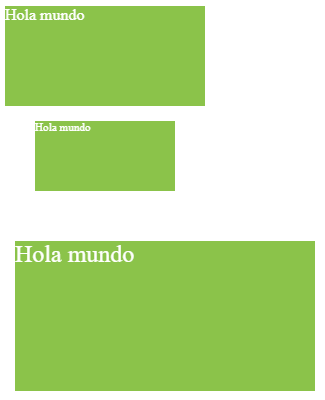
\includegraphics[width=5cm]{ss/scale.png}
\end{figure}

El ejemplo anterior utiliza el mismo valor tanto para el ancho como para el alto, pero se pueden utilizar distintos valores. En caso de que se omita el segundo parámetro, se tomará el valor del primero para el segundo.



\section{Animaciones}


\subsection{Keyframes \& animaciones}

La regla \textbf{keyframes} permite crear animaciones que pueden ser asignadas a un elemento mediante la propiedad \textbf{animation}. Estas animaciones tienen un inicio y un fin, el inicio puede ser la palabra reservada \textbf{from} o el 0\% y el final puede ser la palabra reservada \textbf{to} o el 100\% o se puede navegar a través de estos porcentajes para hacer una animación más detallada.

Puede animar todas las propiedades que desee las veces que sean. Las reglas \textit{keyframes} deben tener un nombre identificativo el cual será el que sea asignado a la propiedad \textit{animation}, como vemos en el siguiente ejemplo:
\begin{lstlisting}
    /* Animación con regla donde cambia el color de fondo. */
    @keyframes example {
        0%  {background-color: red;}
        50%  {background-color: yellow;}
        70%  {background-color: blue;}
        100% {background-color: green;}
    }
\end{lstlisting}

El nombre de la regla es \textit{example}, y cambia el color del fondo del elemento de rojo a amarillo, azul y verde, a través de los distintos porcentajes establecidos, esta animación entonces cambia gradualmente el color de fondo de un elemento.


\subsection{Propiedades de las animaciones}
\begin{itemize}
    \item \textbf{animation-name}: asigna una regla \textit{kewframes} a un elemento.
    \item \textbf{animation-duration}: establece la duración de la animación. Acepta valores en segundos. Si no se establece esta propiedad, la animación no comenzará, esto porque el valor por defecto es 0.
    \begin{lstlisting}
        div {
            animation-name: example;
            animation-duration: 3s;
        }
    \end{lstlisting}
    \item \textbf{animation-timming-function}: cambia la velocidad en la que la transición se crea dentro de la duración establecida. Los valores que acepta son los mismos que la propiedad \textit{transition-timming-function} en la sección \textbf{Transiciones} (\textbf{ease}, \textbf{linear}, \textbf{ease-in}, \textbf{ease-out}, \textbf{ease-in-out} y \textbf{cubic-bezier()}).
    \item \textbf{animation-delay}: agregar un retraso a la animación. Acepta valores en segundos o milisegundos.
    \begin{lstlisting}
        div {
            animation--timming-function: ease-in;
            animation-delay: 1s;
        }
    \end{lstlisting}
    \item \textbf{animation-iteration-count}: determina el número de veces que una animación se repetirá. Acepta valores enteros y la palabra reservada \textbf{infinite}, para repetir indefinidamente una animación. Si utiliza el valor 0, la animación nunca comenzará.
    \item \textbf{animation-direction}: indica el comportamiento de la regla o cómo esta es aplicada. Los valores que acepta son:
    \begin{itemize}
        \item \textit{normal}: la animación se aplica de 0\% a 100\%.
        \item \textit{reverse}: la animación se aplica de 100\% a 0\%.
        \item \textit{alternate}: la animación primero corre hacia adelante, luego hacia atrás, luego hacia adelante.
        \item \textit{alternate-reverse}: la animación primero corre hacia atrás, luego hacia adelante, luego hacia atrás.
    \end{itemize}
\end{itemize}

Dejamos un ejemplo para que lo pruebe y vea cómo se ve la animación:
\begin{lstlisting}
estilos.css
    /* Animación con regla donde el ancho pasa de 0px a 100px. */
    @keyframes colorchange {
        from { width: 0px; }
        to { width: 100px; }
    }
    /* Clase que define las propiedades de la animación con regla en contenedor. */
    .animation {
        animation-name: colorchange;
        animation-duration: 3s;
        animation-timing-function: ease-in;
        animation-delay: 1s;
        animation-iteration-count: infinite;
        animation-direction: reverse;
        height:100px;
        width:0px;
    }

prueba.html
    <div class="animation"></div>
\end{lstlisting}

Puede utilizar el \textbf{acceso directo} de la propiedad \textit{animation} de la siguiente forma:
\begin{center}
    \textit{animation: name duration timming-function delay iteration-count direction}
\end{center}

\section{Filtros}

Los \textbf{Filtros CSS} permiten agregar una capa de efectos gráficos, como desenfoque o cambio de color a un elemento, suelen ser utilizados estos filtros para ajustar el renderizado de imágenes, fondos y bordes. El filtrado de imágenes es útil cuando se requiere tener distintos estilos para una sola imagen; en vez de subir la misma imagen varias veces pero con distinta edición, se puede subir solamente una vez y aplicarle varios filtros con estilos distintos.

Los filtros no están disponibles para Internet Explorer, Edge 12, Safari 5.1 y versiones anteriores del mismo.

Por ejemplo, el método \textit{drop-shadow()} crea una sombra para un elemento, sus parámetros son:
\begin{center}
    \textit{filter: drop-shadow(width height blur color)}
\end{center}

Vemos que esta propiedad tiene los mismos parámetros que \textit{box-shadow}, a diferencia de que no incluye el parámetro \textit{spread}. La \textit{Figura \ref{fig: 57}} tiene el resultado de un ejemplo:
\begin{lstlisting}
estilos.css
    img {
        width: 130px;
        height: 100px;
    }
    /* Filtro de sombra con desenfoque. */
    .dropshadow {
        filter: drop-shadow(5px 9px 2px blue);
    }

prueba.html
    Image<br>
    <img src="http://www.sololearn.com/images/tree.jpg"/>
    <p>Drop Shadow 5px 9px 2px blue<p>
    <img class="dropshadow" src="http://www.sololearn.com/images/tree.jpg"/>
\end{lstlisting}
\begin{figure}[H]
    \centering
    \caption{Método \textbf{drop-shadow()} para agregar una sombra a un elemento}
    \label{fig: 57}
    \includegraphics[width=5cm]{ss/scale.png}
\end{figure}


\subsection{Funciones}

Algunos de los métodos disponibles para los filtros son:
\begin{itemize}
    \item \textbf{blur()}: aplica un efecto de desenfoque a un elemento. Acepta un valor entero, no porcentajes, donde este valor es el radio de píxeles que se mezclan entre sí (un valor mayor crea mayor desenfoque). Si no se escribe un valor en el parámetro, el valor por defecto es 0.
    \item \textbf{brightness()}: ajusta el brillo de un elemento, haciendo que se vea más brillosa u oscura. 0\% es un elemento completamente oscuro, 100\% es un elemento sin cambio alguno y valores mayores al 100\% produce una imagen brillosa. Los valores enteros permitidos van de 0 a 1, cualquier valor negativo simplemente hará la imagen negra.
    \item \textbf{contrast()}: ajusta el contraste de un elemento. 0\% representa un elemento completamente gris, 100\% es el elemento sin cambios, entonces, el contraste se maneja entre valores mayores y menores al 100\%. Los valores enteros permitidos van de 0 a 1, cualquier valor negativo no aplicará un cambio al elemento.
    \item \textbf{drop-shadow()}.
    \item \textbf{grayscale()}: agrega una escala de grises a un elemento. El único parámetro disponible es el porcentaje o valor entero de la escala a aplicar, donde 0\% es el elemento original y 100\% tiene una escala de grises completa. Cualquier valor negativo no hará efecto en el elemento. Los valores enteros permitidos van de 0 a 1.
    \item \textbf{hue-rotate()}: aplica una rotación de tonos (basada en el círculo de colores presente en la \textit{Figura \ref{fig: 58}}) a un elemento. Este método recibe un ángulo como parámetro, 0 y 360 es el color rojo y lo puede ajustar como requiera.
    \item \textbf{invert()}: invierte los colores de un elemento de tal forma que se aplica brillo a zonas oscuras y se oscurecen zonas brillosas. La forma de trabajar este método es el mismo que \textit{grayscale}, sin embargo, acepta valores mayores al 100\%, pero estos no tendrán efecto en el elemento.
    \item \textbf{opacity()}: establece un efecto de transparencia a un elemento. 0\% es el valor para un elemento completamente transparente y 100\% es el elemento original. No acepta valores enteros.
    \item \textbf{saturate()}: controla la saturación de un elemento. El único parámetro disponible es el porcentaje o valor entero de la proporción de saturación a aplicar, donde 0\% es \textbf{completamente insaturada} (escala de grises) y 100\% es el elemento original. Los valores enteros permitidos van de 0 a 1.
    \item \textbf{sepia()}: convierte un elemento a sepia. La forma de trabajar este método es el mismo que \textit{grayscale}, sin embargo, acepta valores mayores al 100\%.
\end{itemize}
\begin{figure}[H]
    \centering
    \caption{El círculo de colores}
    \label{fig: 58}
    \includegraphics[width=5cm]{ss/circle-of-colors.png}
\end{figure}

Mostramos ejemplos de los métodos anteriormente mencionados en las \textit{Figuras \ref{fig: 59}} y \textit{\ref{fig: 60}} respectivamente:
\begin{lstlisting}
estilos.css
    /* Clase para mostrar contenedores uno al lado del otro. */
    .cont {
        display: inline-block;
    }
    /* Clase para contener etiqueta e imagen. */
    .layout {
        display: inherit;
    }
    /* Filtro de escala de grises, rotación de tonos, inversión, saturación y sepia. */
    .grayscale {
        filter: grayscale(100%);
    }
    .hue-rotate {
        filter: hue-rotate(180deg);
    }
    .invert {
        filter: invert(70%);
    }
    .saturate {
        filter: saturate(25%);
    }
    .sepia {
        filter: sepia(70%);
    }

prueba.html
    <div class="cont">
        <div class="layout">
            <p>Original</p>
            <img src="http://www.sololearn.com/images/tree.jpg" alt="">
        </div>
        <div class="layout">
            <p>Grayscale</p>
            <img src="http://www.sololearn.com/images/tree.jpg" alt="" class="grayscale">
        </div>
        <div class="layout">
            <p>Hue-rotate</p>
            <img src="http://www.sololearn.com/images/tree.jpg" alt="" class="hue-rotate">
        </div>
        <div class="layout">
            <p>Invert</p>
            <img src="http://www.sololearn.com/images/tree.jpg" alt="" class="invert">
        </div>
        <div class="layout">
            <p>Saturate</p>
            <img src="http://www.sololearn.com/images/tree.jpg" alt="" class="saturate">
        </div>
        <div class="layout">
            <p>Sepia</p>
            <img src="http://www.sololearn.com/images/tree.jpg" alt="" class="sepia">
        </div>
    </div>
\end{lstlisting}
\begin{figure}[H]
    \centering
    \caption{Conjunto 1 de ejemplos de filtros CSS}
    \label{fig: 59}
    \includegraphics[width=14cm]{ss/filter-examples-1.png}
\end{figure}
\begin{lstlisting}
estilos.css
    /* Clase para mostrar contenedores uno al lado del otro. */
    .cont {
        display: inline-block;
    }
    /* Clase para contener etiqueta e imagen. */
    .layout {
        display: inherit;
    }
    /* Filtros de opacidad, brillo, contraste y desenfoque. */
    .opacity {
        filter: opacity(70%);
    }
    .brightness {
        filter: brightness(50%);
    }
    .contrast {
        filter: contrast(140%);
    }
    .blur {
        filter: blur(10px);
    }

prueba.html
    <div class="cont">
        <div class="layout">
            <p>Original</p>
            <img src="http://www.sololearn.com/images/tree.jpg" alt="">
        </div>
        <div class="layout">
            <p>Opacity</p>
            <img src="http://www.sololearn.com/images/tree.jpg" alt="" class="opacity">
        </div>
        <div class="layout">
            <p>Brightness</p>
            <img src="http://www.sololearn.com/images/tree.jpg" alt="" class="brightness">
        </div>
        <div class="layout">
            <p>Contrast</p>
            <img src="http://www.sololearn.com/images/tree.jpg" alt="" class="contrast">
        </div>
        <div class="layout">
            <p>Blur</p>
            <img src="http://www.sololearn.com/images/tree.jpg" alt="" class="blur">
        </div>
    </div>
\end{lstlisting}
\begin{figure}[H]
    \centering
    \caption{Conjunto 2 de ejemplos de filtros CSS}
    \label{fig: 60}
    \includegraphics[width=14cm]{ss/filter-examples-2.png}
\end{figure}


\subsection{Usando múltiples filtros}

Se pueden aplicar varios estilos a un solo elemento, simplemente se separan por espacios, como se ve en la \textit{Figura \ref{fig: 61}}:
\begin{lstlisting}
estilos.css
    .filtered {
        /* Agrega filtros de saturación, sombra y desenfoque. */
        filter: saturate(30%) drop-shadow(5px 9px 2px gray) blur(1px);
    }

prueba.html
    <img class="original" src="http://www.sololearn.com/images/tree.jpg">
    <img class="filtered" src="http://www.sololearn.com/images/tree.jpg">
\end{lstlisting}
\begin{figure}[H]
    \centering
    \caption{Uso de múltiples filtros CSS}
    \label{fig: 61}
    \includegraphics[width=10cm]{ss/filter-multiple.png}
\end{figure}


% Fin del documento.
\end{document}